%%%%%%%%%%%%%%%%%%%%%%%%%%%%%%%%%%%%%%%%%%%%%%%%%%%%%%%%%%%%%%%%%%%%%%%%%%%%%%%%
%2345678901234567890123456789012345678901234567890123456789012345678901234567890
%        1         2         3         4         5         6         7         8

\documentclass[twocolumn,10pt]{asme2ej}  % Comment this line out if you need a4paper

%\documentclass[a4paper, 10pt, conference]{ieeeconf}      % Use this line for a4 paper

%\IEEEoverridecommandlockouts                              % This command is only needed if 
% you want to use the \thanks command

%\overrideIEEEmargins                                      % Needed to meet printer requirements.

% See the \addtolength command later in the file to balance the column lengths
% on the last page of the document

% The following packages can be found on http:\\www.ctan.org
%\usepackage{graphicx}
\usepackage{graphics} % for pdf, bitmapped graphics files
\usepackage{epsfig} % for postscript graphics files
\usepackage{subcaption}
\usepackage[noadjust]{cite}
%\usepackage{mathptmx} % assumes new font selection scheme installed
%\usepackage{times} % assumes new font selection scheme installed
\usepackage{amsmath,amssymb,amsfonts,mathrsfs} % assumes amsmath package installed
\usepackage{algorithm,algpseudocode}
%\usepackage{booktabs}
\usepackage{balance}
\usepackage{tcolorbox}

% format for theorems etc.
\newtheorem{thm}{\bfseries Theorem}
\newtheorem{lem}{\bfseries Lemma}
\newtheorem{cor}{\bfseries Corollary}
\newtheorem{prop}{\bfseries Proposition}
\newtheorem{rem}{\bfseries Remark}

% format for argmin, argmax
\newcommand{\argmax}{\operatornamewithlimits{argmax}}

% format for cross-reference
\usepackage[capitalize]{cleveref}
\crefname{equation}{eq.}{eq.}
\Crefname{equation}{Eq.}{Eq.}
\crefname{thm}{theorem}{theorems}
\Crefname{thm}{Theorem}{Theorems}
\crefname{lem}{lemma}{lemmas}
\Crefname{lem}{Lemma}{Lemmas}
\crefname{cor}{corollary}{corollaries}
\Crefname{cor}{Corollary}{Corollaries}
\crefname{prop}{proposition}{propositions}
\Crefname{prop}{Proposition}{Propositions}
\crefname{rem}{remark}{remarks}
\Crefname{rem}{Remark}{Remarks}

% =====Macros for this manuscript===== %
\newcommand{\proto}{FIFO}
\newcommand{\lb}{\left\lbrace}
\newcommand{\rb}{\right\rbrace}
\newcommand{\X}{X}
\newcommand{\Z}{Z}
\newcommand{\zb}{\mathbf{z}}
\newcommand{\B}{\mathcal{B}}
\newcommand{\Q}{\mathcal{Q}}
\newcommand{\K}{\mathcal{K}}
\newcommand{\xg}{x^g}
\newcommand{\fc}{frequently jointly strongly connected}
\newcommand{\thi}{^\text{th}}
\newcommand{\dnbhd}{direct neighbors}
\newcommand{\anbhd}{accessible neighbors}

%=====todonotes===== %
\usepackage{todonotes}
\usepackage{soul}
\definecolor{smoothgreen}{rgb}{0.7,1,0.7}
\sethlcolor{smoothgreen}

\newcommand{\todopara}[1]{\vspace{0px} %
	\todo[inline, color=black!10]{\textbf{[Paragraph:]} {#1}} %
}
\newcommand{\todonote}[1]{\vspace{0px} %
	\todo[inline, color=green!30]{\textbf{[Note:]} {#1}} %
}
\newcommand{\todoQ}[1]{\vspace{0px} %
	\todo[inline, color=orange!50]{\textbf{[Note:]} {#1}} %
}
\newcommand{\todohere}[1]{\hl{(\textbf{TODO:} #1)}}

\newcommand{\hidetodos}{
	\renewcommand{\todopara}[1]{}
	\renewcommand{\todonote}[1]{}
	\renewcommand{\todoQ}[1]{}
	\renewcommand{\todohere}[1]{}
}

\title{\LARGE \bf
Estimation of Moving Targets Using Distributed Bayesian Filter Under Dynamically Changing Networks}
	%Distributed Bayesian Filter Under Dynamically Changing Interaction Topologies}


%%% first author
\author{Chang Liu
	\affiliation{		
		Department of Mechanical Engineering\\
		University of California, Berkeley\\
		Berkeley, CA 94720\\
		Email: changliu@berkeley.edu
	}	
}
%\thanks{The first two authors have equally contributed to this research.}

%%% second author
%%% remove the following entry for single author papers
%%% add more entries for additional authors
\author{Shengbo Eben Li\thanks{Address all correspondence to this author.}
	\affiliation{Department of Automotive Engineering\\ 
		Tsinghua University\\
		Beijing, China 100084\\
		Email: lisb04@gmail.com
	}
}

%%% third author
%%% remove the following entry for single author papers
%%% add more entries for additional authors
\author{J. Karl Hedrick
	\affiliation{
		Department of Mechanical Engineering\\
		University of California, Berkeley\\
		Berkeley, CA 94720\\
		Email: khedrick@me.berkeley.edu
	}
}

%\author{Chang Liu$^{1}$, Shengbo Eben Li$^{2}$ and J. Karl Hedrick$^{3}$% <-this % stops a space
%	\thanks{*The first two authors, C. Liu and S. Li, have equally contributed to this research.}% <-this % stops a space
%	\thanks{$^{1}$C. Liu is with the Vehicle Dynamics \& Control Lab, Department of Mechanical Engineering, University of California, Berkeley, Berkeley, CA 94709, USA. Email: {\tt\small changliu@berkeley.edu}}%
%	\thanks{$^{2}$S. Eben Li is with the Department of Automotive Engineering, Tsinghua University, Beijing, 100084, China. He has worked at the Department of Mechanical Engineering, University of California, Berkeley as a visiting scholar. Email: {\tt\small lisb04@gmail.com}}%
%	\thanks{$^{3}$J. K. Hedrick is with the Vehicle Dynamics \& Control Lab, Department of Mechanical Engineering, University of California, Berkeley, Berkeley, CA 94709, USA. Email: {\tt\small khedrick@me.berkeley.edu}}%
%}


\begin{document}
	
	%\hidetodos % hide all todos 
	
	\maketitle
	\thispagestyle{empty}
	\pagestyle{empty}
	
	%\setlength{\belowcaptionskip}{-10pt} % set the spacing between figure and text
	
	%%%%%%%%%%%%%%%%%%%%%%%%%%%%%%%%%%%%%%%%%%%%%%%%%%%%%%%%%%%%%%%%%%%%%%%%%%%%%%%%
	\begin{abstract}
		This paper presents a distributed Bayesian filtering (DBF) method for a network of multiple unmanned ground vehicles (UGVs) under dynamically changing interaction topologies. The information exchange among UGVs relies on a measurement dissemination scheme, called Latest-In-and-Full-Out (\proto) protocol. Different from statistics dissemination approaches that transmit posterior distributions or likelihood functions, each UGV under \proto only sends a buffer that contains latest available measurements to neighboring nodes, which significantly reduces the transmission burden between each pair of UGVs to scale linearly with the size of the network.
		Under the condition that the union of undirected switching topologies is connected frequently enough,
		\proto can disseminate observations over the network within finite time. 
		The \proto-based DBF algorithm is then derived to estimate individual probability density function (PDF) for target localization in a static environment. The consistency of this algorithm is proved that each individual estimate of target position converges in probability to the true target position.
		The effectiveness of this method is demonstrated by comparing with consensus-based distributed filters and the centralized filter in simulations.
	\end{abstract}
	
	\section{INTRODUCTION}
	
%	Unmanned ground vehicles (UGV) that operate without on-board operators have been used for many applications that are inconvenient, dangerous, or impossible to human. 
	Estimation using a group of networked UGVs has been widely utilized to collectively measure environment status \cite{hedrick2011tools}, such as intruder detection \cite{chamberland2007wireless}, signal source seeking \cite{atanasov2015distributed}, and pollution field estimation \cite{madhag2017distributed},
	due to its merits on low cost, high efficiency, and good reliability.
	The commonly adopted estimation approaches include the Kalman Filter, extended Kalman filter, and particle filter \cite{thrun2005probabilistic}, and
%	Several techniques have been developed for distributed estimation, including distributed linear Kalman filter (DKF) \cite{2005distributed}, distributed extended Kalman filter \cite{madhavan2004distributed}, and distributed particle filter \cite{gu2007distributed}. 
	the most generic scheme might be the Bayesian filter because of its applicability for nonlinear systems with arbitrary noise distributions \cite{bandyopadhyay2014distributed,julian2012distributed}.
	In fact, a Bayesian filter can be reduced to different methods in certain conditions.
	For example, under the assumption of linearity and Gaussian noise, a Bayesian filter can be reduced to the Kalman filter \cite{chen2003bayesian}; 
	\textcolor{\revcol}{for general nonlinear systems, a Bayesian filter can be numerically implemented as a particle filter \cite{chen2003bayesian}}.
%	due to the advantage in computation \cite{chen2003bayesian}.
	Because of this generality, this study focuses on its networked variant, \textcolor{\revcol}{and use it for tracking targets via local communication between neighboring UGVs.} % under dynamically changing interaction topologies.
	
	The interaction topology \cite{zheng2016stability,zheng2017distributed} plays a central role on the design of networked Bayesian filter, of which two types are widely investigated in literature: centralized filters and distributed filters.
	In the former, local statistics estimated by each agent is transmitted to a single fusion center, where a global posterior distribution is calculated at each filtering cycle \cite{zuo2006bandwidth,vemula2006target}. 
	In the latter, each agent individually executes distributed estimation and the agreement of local estimates is achieved by certain consensus strategies \cite{jadbabaie2003coordination,ren2005consensus,olfati2007consensus}.
	In general, the distributed filters are more suitable in practice since they do not require a fusion center with powerful computation capability and are more robust to changes in network topology and link failures. 
	So far, the distributed filters have two mainstream schemes in terms of the transmitted data among agents, i.e., \textit{statistics dissemination} (SD) and \textit{measurement dissemination} (MD). 
	In the SD scheme, each agent exchanges statistics, such as posterior distributions and likelihood functions, within neighboring agents \cite{hlinka2013distributed}. 
	In the MD scheme, instead of exchanging statistics, each agent sends sensor measurements to neighboring agents. 
	
%	The pioneering work of statistics dissemination scheme can date back to the 80s of last century \todohere{reference}. 
%	Later, \todohere{reference} have considerably advanced the study of this scheme in the field of distributed estimation. 
	The statistics dissemination scheme has been widely investigated during the last decade, especially in the field of signal processing, network control, and robotics.
	Madhavan et al. (2004) presented a distributed extended Kalman filter for nonlinear systems \cite{madhavan2004distributed}. 
	This filter was used to generate local terrain maps by using pose estimates to combine elevation gradient and vision-based depth with environmental features. 
	Olfati-Saber (2005) proposed a distributed linear Kalman filter (DKF) for estimating states of linear systems with Gaussian process and measurement noise \cite{2005distributed}. 
	Each DKF used additional low-pass and band-pass consensus filters to compute the average of weighted measurements and inverse-covariance matrices. 
	Gu (2007) proposed a distributed particle filter for Markovian target tracking over an undirected sensor network \cite{gu2007distributed}. Gaussian mixture models (GMM) were adopted to approximate the posterior distribution from weighted particles and the parameters of GMM were exchanged via average consensus filter. 
	Hlinka et al. (2012) proposed a distributed method for computing an approximation of the joint (all-sensors) likelihood function by means of weighted-linear-average consensus algorithm when local likelihood functions belong to the exponential family of distributions \cite{hlinka2012likelihood}. Saptarshi et al. (2014) presented a Bayesian consensus filter that uses logarithmic opinion pool for fusing posterior distributions of the tracked target \cite{bandyopadhyay2014distributed}. Other examples can be found in \cite{julian2012distributed} and \cite{beaudeau2012target}. 
	
	Despite the popularity of statistics dissemination, exchanging statistics can cause high communication burden if the environment to be detected is relatively large in space and complicated in structure. 
	One remedy is to approximate statistics with parametric models, e.g., Gaussian Mixture Model \cite{sheng2005distributed}, which can reduce communication burden to a certain extent. 
	However, such manipulation increases the computation burden of each agent and sacrifices filtering  accuracy due to approximation.
	The measurement dissemination scheme is an alternative solution to address the issue of exchanging large-scale statistics. 
	An early work on measurement dissemination was done by Coates et al. (2004), who used adaptive encoding of observations to minimize communication overhead \cite{coates2004distributed}. Ribeiro et al. (2006) exchanged quantized observations along with error-variance limits considering more pragmatic signal models \cite{ribeiro2006bandwidth}.
	A recent work was conducted by Djuric et al. (2011), who proposed to broadcast raw measurements to other agents, and therefore each agent has a complete set of observations of other agents for executing particle filtering \cite{djuric2011non}.  
	A shortcoming of aforementioned works is that their communication topologies are assumed to be a fixed and complete graph that every pair of distinct agents is constantly connected by a unique edge. 
	In many real applications, the interaction topology can be time-varying due to unreliable links, external disturbances or range limits \cite{xiao2008asynchronous,gao2016robust}.
	In such cases, dynamically changing topologies can cause random packet loss, variable transmission delay, and out-of-sequence measurement (OOSM) issues \cite{xia2009networked}, thus decreasing the performance of distributed estimation.
%	, and even leading to inconsistency and non-consensus. 
	Leung et al. (2010) has explored a decentralized Bayesian filter for dynamic robot networks \cite{leung2010decentralized} in order to achieve centralized-equivalent filtering performance.
	However, it requires the communication of both measurements and statistics, which can still incur large communication overhead.
	
	\textcolor{\revcol}{
	This paper proposes a distributed Bayesian filtering (DBF) method that only uses measurement dissemination for a group of networked UGVs with dynamically changing interaction topologies. 
	In our previous works \cite{liu2017measurement,liu2016distributed,liu2017distributed}, we have proposed a Latest-In-and-Full-Out (LIFO) protocol for measurement exchange and developed a corresponding DBF algorithm.
%	However, it only applies to static targets with simple binary sensor model.
	However, it is only applicable to either tracking moving targets when the interaction topology is time-invariant or to localizing static targets.
	In this work, we substantially extend the previous works and make the following contributions:
	(1) We introduce a new protocol called the Full-In-and-Full-Out (\proto) that allows each UGV to broadcast a history of measurements to its neighbors via single hopping, enabling the localization and tracking of targets using general nonlinear sensor models under time-varying topologies. 
	(2) We propose the 
	\textit{{\fc ness}} condition of the interaction topology and show that, under this condition, {\proto} can disseminate UGVs' measurements over the network within a finite time.
	(3) We develop a FIFO-based distributed Bayesian filter (FIFO-DBF) for each UGV to implement locally.
	A track list is designed to reduce the computational complexity of FIFO-DBF and the communication burden. 
	The FIFO-DBF can avoid the OOSM issue.
	(4) We prove the consistency of FIFO-DBF: each UGV's estimate of target position converges in probability to the true target position asymptotically if the interaction topologies are \textit{\fc.}}
	
	
	The rest of this paper is organized as follows: 
	\Cref{sec:prob} formulates the target tracking problem using multiple UGVs;
	\Cref{sec:\proto} proposes the {\proto} protocol for measurement dissemination in dynamically changing interaction topologies;
	\Cref{sec:\proto-dbf} introduces the FIFO-DBF algorithm and the track list;
	\Cref{sec:consist_proof} proves the consistency of FIFO-DBF;
%	 where the consistency of estimation is proved;
	\Cref{sec:sim} presents simulation results and \Cref{sec:conclu} concludes the paper.
	\section{Problem Formulation}\label{sec:prob}
\begin{figure}%[thpb]
	\centering
	\includegraphics[width=0.45\textwidth]{figures/scenario}
	\caption{Target tracking scenario. The interaction topology is dynamically changing and UGVs can only communicate with neighboring UGVs.}
	\label{fig:scenario}
	%		\vspace{-1em}]
\end{figure}
%	\section{\proto Protocol for Dynamically Changing Interaction Topologies}\label{sec:lifo}
	Consider a network of $N$ UGVs in a bounded two-dimensional space $S$, as shown in \cref{fig:scenario}.
	The interaction topology can be dynamically changing due to limited communication range, varying team formation or link failure.
	Each UGV is equipped with a sensor for target detection. 
	Due to the limit of communication range, each UGV can only exchange sensor measurements with its local neighbors. 
%	The Bayesian filter is run locally on each UGV based on its own measurements and the received measurements from other UGVs to estimate the target position in $S$.
	Every UGV locally runs a Bayesian filter to estimate the target position in $S$ utilizing its own measurements and the received measurements from other UGVs. 
	Since this work is focused on the distributed Bayesian filter for target localization, we assume that UGVs' states are accurately known.
%	An illustration of the scenario is shown in \cref{fig:scenario}.
	
	\subsection{Target and Sensor Model}
	%Probabilistic Model of Binary Sensor}
	%In this paper, distributed Bayesian filter is used to estimate the true target position by a network of binary sensors.
	The target motion uses a stochastic discrete-time model: % that can be described by
	
	\begin{equation}
		\small
		\label{eqn:tar_motion_model}
		\xg_{k+1}=f(\xg_k,v_k), %,u^g_k
		%x_{k+1}=A_kx_k+B_ku^g_k+\epsilon,
	\end{equation}\normalsize
	where the superscript $g$ represents the target and $\xg_k\in S$ is the target position at time $k$;
	$v_k$ is the white process noise.
	% and $u^g_k$ is the target control input.
	%$A_k\in\mathbb{R}^{2\times 2},\;B_k\in\mathbb{R}^{2\times 2}$ and $\epsilon$ denotes the process noise.
	
	%Each UGV constantly measures the target position and the 
	The sensor measurement is described by a stochastic model:
	\small\begin{equation}\label{eqn:meas_model}
		z^i_k = h_i(\xg_k,x^i_k,w^i_k),
	\end{equation}\normalsize
	where the superscript $i\in\left\lbrace 1,\dots,N\right\rbrace$ represents the index of the UGV; $x^i_k\in S$ is the sensor position and $w^i_k$ is the white measurement noise.
	% $x^i_k=[x^i_k;\theta^i_k]$ represents the sensor state, consisting of the sensor position $x^i_k$ and direction $\theta^i_k$.
	The measurement function $h_i$ depends on the type of the sensor. 
	%Let $\mathcal{F}(x^i_k)$ denote the sensor's sensing domain, 
	
	The conditional probability, $P(z^i_k|x^g_k;x^i_k)$, of obtaining a certain measurement $z^i_k$ conditioning on the target and sensor states is critical to designing the Bayesian filter \cite{thrun2005probabilistic}. 
%	We define $P(z^i_k|x^g_k;x^i_k)$ as this conditional probability.
%	 of $z^i_k$ given the sensor state $x^i_k$ and the target state $\xg_k$. 
	It also depends on the distribution of the measurement noise.
	For example, if $w^i_k$ is an additive, zero-mean Gaussian white noise with covariance $\Gamma_k^i$, then, according to \Cref{eqn:meas_model}, $P(z^i_k|x^g_k;x^i_k)$ can be described as
	\small\begin{equation*}%\label{eqn:prob_sensor3}
		P(z^i_k|x^g_k;x^i_k)=\mathcal{N}(h_i(\xg_k,x^i_k),\Gamma_k^i).
	\end{equation*}\normalsize
	For non-Gaussian noise distributions, such as the Poisson noise or Cauchy noise \cite{kitagawa1996monte}, $P(z^i_k|x^g_k;x^i_k)$\footnote{For the purpose of simplicity, we will not explicitly write the parameter $x^{i}_k$ in $P(z^i_k|x^g_k;x^i_k)$ for the rest of the paper.} can also be similarly defined.
	It should be noted that, the approach presented in this work does not rely on the specific distribution of the noise.
	
	The $h_i$ for several typical sensors are defined as follows \cite{bishop2010optimality}:
	
	\textbf{Range-only sensors:} 
	%when the target is within the sensor's sensing domain, 
	$h_i$ only depends on the relative Euclidean distance between the sensor and the target:
	%\begin{subequations}
	%	\begin{align}
	\small\begin{equation*}%\label{eqn:ran_only}
		h_i(\xg_k,x^i_k)=\|\xg_k-x^i_k\|_2,
	\end{equation*}	\normalsize
	%\begin{equation}\label{eqn:ran_only}
	%h_i(\xg_k,w^i_k;x^i_k)=
	%\begin{cases}
	%\|\xg_k-x^i_k\|_2+w^i_k\; &\text{if}\, \xg_k\in\mathcal{F}(x^i_k)\\
	%\emptyset\; &\text{if}\, \xg_k\notin\mathcal{F}(x^i_k)
	%\end{cases},
	%\end{equation}		
	where $\|\cdot\|_2$ is the Euclidean distance in $S$.
	%		w^i_k&\sim\mathcal{N}(0,\sigma^i),
	%	\end{align}
	%\end{subequations}
	
	\textbf{Bearing-only sensors:} 
	%when the target is within the sensor's sensing domain, 
	$h_i$ only depends on the relative bearing between the sensor and the target:
	\small\begin{equation*}
		h_i(\xg_k,x^i_k)=\measuredangle (\xg_k-x^i_k),
	\end{equation*}\normalsize
	%\begin{equation}
	%h_i(\xg_k,w^i_k;x^i_k)=
	%\begin{cases}
	%\measuredangle (\xg_k-x^i_k)+w^i_k\; &\text{if}\, \xg_k\in\mathcal{F}(x^i_k)\\
	%\emptyset\; &\text{if}\, \xg_k\notin\mathcal{F}(x^i_k)
	%\end{cases},
	%\end{equation}
	where $\measuredangle$ denotes the angle from the sensor to the target.
	
	\textbf{Range-bearing sensors:} $h_i$ includes both the relative distance and bearing: % between the sensor and the target:
	\small\begin{equation*}
		h_i(x^g_k,x^i_k)=x^g_k-x^i_k.
	\end{equation*}\normalsize
	
%	\subsection{Target and Sensor Model}
%	The target motion takes a deterministic discrete-time model:	
%	\begin{equation}
%		\small
%		\label{eqn:tar_motion_model}
%		x^g_{k+1}=f(x^g_k),
%	\end{equation}\normalsize
%	where $x^g_k\in \mathbb{R}^{2}$ denotes the target position at time $k$; $u^g_k$ represents the control input of the target.
%	
%	Each UGV constantly measures the target position and the sensor measurement of $i\thi$ UGV can be described by a stochastic model:
%	\begin{equation}
%		z^i_k = g_i(x^g_k,w^i_k;y^i_k),
%	\end{equation}
%	where $w^i_k$ is the white measurement noise and $y^i_k=[x^i_k;\theta^i_k]$ represents the sensor state, consisting of the sensor position $x^i_k$ and direction $\theta^i_k$.
%	$g_i$ depends on the type of the sensor. Let $\mathcal{F}(y^i_k)$ denote the sensor field of view (FOV), $g_i$ for several typical sensor types can be defined as follows:
%	
%	\textbf{Range-only sensors:} when the target is within the sensor's FOV, the measurement only depends on the relative distance between the sensor and the target.
%	\begin{equation*}%\label{eqn:ran_only}
%		h_i(\xg_k,x^i_k)=\|\xg_k-x^i_k\|_2,
%	\end{equation*}	
%%	\begin{equation}
%%		g_i(x^g_k,w^i_k;x^i_k)=
%%		\begin{cases}
%%			\|x^g_k-x^i_k\|_2+w^i_k\; &\text{if}\, x^g_k\in\mathcal{F}(y^i_k),\\
%%			\emptyset\; &\text{if}\, x^g_k\notin\mathcal{F}(y^i_k).
%%		\end{cases}
%%	\end{equation}
%	
%	\textbf{Bearing-only sensors:} when the target is within the sensor's FOV, the measurement only depends on the relative bearing between the sensor and the target.
%	\begin{equation}
%		g_i(x^g_k,w^i_k;x^i_k)=
%		\begin{cases}
%			\measuredangle (x^g_k-x^i_k)+w^i_k\; &\text{if}\, x^g_k\in\mathcal{F}(y^i_k),\\
%			\emptyset\; &\text{if}\, x^g_k\notin\mathcal{F}(y^i_k).
%		\end{cases}
%	\end{equation}
%	
%	\textbf{Range-bearing sensors:} $h_i$ includes both the relative distance and bearing: % between the sensor and the target:
%	\begin{equation*}
%		h_i(x^g_k,x^i_k)=x^g_k-x^i_k.
%	\end{equation*}
%	
%%	\textbf{Range-bearing sensors:} when the target is within the sensor's FOV, the measurement is the relative distance and bearing between the sensor and the target.
%%	\begin{equation}
%%		g_i(x^g_k,w^i_k;x^i_k)=
%%		\begin{cases}
%%			x^g_k-x^i_k+w^i_k\; &\text{if}\, x^g_k\in\mathcal{F}(y^i_k),\\
%%			\emptyset\; &\text{if}\, x^g_k\notin\mathcal{F}(y^i_k).
%%		\end{cases}
%%	\end{equation}
%		
%	A probabilistic sensor model that describes the conditional probability of a certain measurement given sensor and target state is a key component for Bayesian filtering.
%	We define a likelihood function to represent the probability of the target being detected by a sensor:
%	\small\begin{equation}\label{eqn:prob_sensor1}
%		p^i_{1,k}=P(z^i_k\neq\emptyset|x^g_k;x^i_k)\in \left[0,1\right],\; x^g_k\in S,
%	\end{equation}\normalsize
%	where $x^i_k$ is the $i\thi$ sensor's position.
%	%; $X^g$ represents the set of all possible target positions.
%	Correspondingly, the likelihood function for no target being detected is:
%	\small\begin{equation}\label{eqn:prob_sensor0}
%		p^i_{0,k}=P(z^i_k=\emptyset|x^g_k;x^{i}_k)=1-p^i_{1,k}.
%	\end{equation}\normalsize
%	%\Cref{eqn:bin_sensor} actually defines a binary sensor model parameterized by $x^g_k$ and $x^R_k$.
%	
%	The combination of \Cref{eqn:prob_sensor1} and \Cref{eqn:prob_sensor0} forms the probabilistic model for a sensor.
%	If $w^i_k$ is a zero-mean Gaussian white noise, then the probabilistic sensor model can be described as
%	\begin{equation}		
%		\begin{cases}
%			p^i_{1,k}\sim\mathcal{N}(\bar{z}^i_k,\Sigma^i_k) & \text{if}\,x^g_k\in\mathcal{F}(y^i_k)\\
%			p^i_{1,k}=0 & \text{if}\,x^g_k\in\mathcal{F}(y^i_k),
%		\end{cases}
%	\end{equation}
%	where $\bar{z}^i_k$ is the nominal value of the measurement and equals $\|x^g_k-x^i_k\|$ and $\measuredangle(x^g_k-x^i_k)$ for range-only and bearing-only sensors, correspondingly.
%	
%	Consequently,
%	\begin{equation}
%		p^i_{0,k}=
%		\begin{cases}
%			0 & \text{if}\,x^g_k\in\mathcal{F}(y^i_k)\\
%			1 & \text{if}\,x^g_k\in\mathcal{F}(y^i_k).
%		\end{cases}
%	\end{equation}
	
%	For the purpose of simplicity, we will not explicitly write $x^{i}_k$ in the sensor model (\Cref{eqn:prob_sensor1,eqn:prob_sensor0}) for the rest of the paper.
	
	\begin{rem}
		Given the knowledge of current target and UGV positions, the current measurement by each UGV can be considered conditionally independent from its own past measurements and those by other UGVs \cite{bourgault2003optimal}.
	\end{rem}
	
%	\begin{rem} 
%		The proposed {\proto} protocol and the consistency property to be described in \cref{sec:\proto-dbf} are applicable for general sensors, not limited to the ones described in this section. In addition, they do not rely on the Gaussian noise assumption.
%	\end{rem}
	
	\subsection{Graphical Model of Interaction Topology}
	%The UGV network is always assumed to be connected, i.e., there exists a path, either direct or indirect, between every pair of UGVs.
	%Under this assumption, consider an undirected and fixed graph 
	We consider a simple\footnote{A (directed/undirected) graph $G=(V,E)$ is \textit{simple} if it has no self-loops (i.e., $\left( i,j\right)\in E\,\text{only if } i\neq j$) or multiple edges with the same source and target nodes (i.e., $E$ only contains distinct elements).} graph $G=(V,E)$ to represent the interaction topology of N networked UGVs, where the vertex set $V=\left\lbrace 1,\dots,N\right\rbrace $ represents the index set of UGVs and $E=V\times V$ denotes the edge set. 
	For the purpose of clarity and generalizability, we use directed graphs to describe our approach in this work.
	However, the approach can conveniently apply to undirected graphs, which can be treated as bidirectional directed graphs.
	
	The \textit{adjacency matrix} $A=\left[ a_{ij}\right] $ of the graph $G$ describes the interaction topology:
	\small\begin{equation*}
		a_{ij}=\begin{cases}
			1& \text{if}\;\left(i,j\right)\in E\\
			0& \text{if}\;\left(i,j\right)\notin E
		\end{cases},
	\end{equation*} \normalsize
	where $a_{ij}$ is the entry on the $i\thi$ row and $j\thi$ column of the adjacency matrix. 
	The notation $a_{ij}=1$ indicates that the $i\thi$ UGV can directly communicate to the $j\thi$ UGV and $a_{ij}=0$ indicates no direct communication from $i$ to $j$.
%	 a communication link exists from the $i\thi$ to $j\thi$ UGV and $m_{ij}=0$ indicates no communication from $i$ to $j$.
	 A directed graph is \textit{strongly connected} if there is a directed path connecting any two arbitrary vertices in $V$\footnote{An undirected graph with this property is called a \textit{connected} graph.}.
%	\cref{fig:com_topo} illustrates three types of typical simple directed topologies: ring \cite{lawton2003decentralized}, line \cite{liu2010simple}, and star \cite{thatte2008sensor}. 
%	All of them are represented by simple and undirected graphs.
	
%	The interaction topology can be dynamically changing due to limited communication range, varying team formation or link failure.
%	Let $\bar{G}=\left\lbrace G_1,G_2,\dots,G_L\right\rbrace $ denote the set of all possible simple and undirected graphs defined for the network of UGVs.
%	Let $\bar{G}$ denote the set of all possible simple and undirected graphs defined for the network of UGVs.
%	Let $\bar{G}$ denote the set of all possible simple directed graphs\footnote{For undirected graphs, we consider the set of simple undirected graphs.} defined over the network of UGVs.
%	It is easy to know that $\bar{G}$ has finite elements.
%	The adjacency matrix associated with a graph $G_l\in\bar{G}$ is denoted as $A_l=[a^l_{ij}]$.	
	Define the \textit{union} of a collection of simple directed graphs\footnote{For undirected graphs, we consider the set of simple undirected graphs.} \small$\left\lbrace G_{i_1},G_{i_2},\dots,G_{i_l} \right\rbrace$\normalsize as the graph with the vertices in $V$ and the edge set given by the union of edge sets of \small$G_{i_j},\,j=1\dots,l$\normalsize.
	Such collection is \textit{jointly strongly connected} if the union of its members forms a strongly connected graph\footnote{For undirected graphs, such collection is \textit{jointly connected} \cite{jadbabaie2003coordination}.}.
%	We define the concept of neighbors in a UGV network.
%	\todohere{note that the definition for neighbor here means neighbors who can receive robot $i$'s CB, so it's outbound neighbors for directed graph.}
	We define the \textit{\dnbhd} of $i\thi$ UGV under topology $G_{l}$ as the set \small$\mathcal{N}_i(G_{l})=\left\lbrace j|a^l_{ij}=1,\,j\in V\right\rbrace $\normalsize. %\left\lbrace1,\dots,N \right\rbrace 
	All UGVs in $\mathcal{N}_i(G_{l})$ can directly receive information from the $i\thi$ UGV via the single hopping.
%	The \textit{\anbhd} is defined as $\mathcal{Q}_i(G_{l})$ that contains indices of UGVs whose information can be received by the $i\thi$ UGV, possibly via multi-hopping, given a specific data exchange protocol and the interaction topology $G_{l}$. 
%	Note that in general $\mathcal{N}_i(G_{l})\subseteq\mathcal{Q}_i(G_{l})$.
	%but when only single-hopping is allowed, $\mathcal{N}_i=\mathcal{Q}_i$. 
	\section{Full-In-and-Full-Out (\proto) Protocol}\label{sec:\proto}	
	This study proposes a Full-In-and-Full-Out (\proto) protocol for measurement exchange in time-varying topologies.
%	In our previous work, we proposed a Latest-In-and-Full-Out (LIFO) protocol and can be used for time-invariant topologies.
%	{\proto} is suitable for time-varying topologies.
%	Let $y_k^i=\left\lbrace x^i_k,z^i_k\right\rbrace$ and $Y^i_{\K}=\left\lbrace y_{k}^i|k\in \K\right\rbrace$, where $\K$ is an index set of time steps.
	Let $Y^i_{\K}=\lb \left[x^i_k,z^i_k\right]|k\in \K\rb$ 
	% $Y^i_{\K^{i,j}_k}=\lb \left[x^{i,j}_t,z^{i,j}_t\right]|t\in \K^{i,j}_k\rb$
	be the set of state-measurement pairs of robot $i$, where $\K$ is an index set of time steps.
	Each UGV contains a communication buffer (CB) that stores state-measurement pairs 
%	consisting of measurements and the corresponding states 
	of all UGVs:
	\begin{equation*}		
		\B^i_k=\left[ Y^1_{\K^{i,1}_k},\dots,Y^N_{\K^{i,N}_k}\right],
%		\mathbf{z}^{CB,i}_k=\left[ z^1_{k^i_1},\dots,z^N_{k^i_N}\right]
	\end{equation*}
%	where $z^j_{k^i_j}$ represents the observation made by ${j\thi}$ UGV at time $k^i_j$. 
	where $\B^i_k$ is the CB of $i\thi$ UGV at time $k$ and $\K^{i,j}_k (j\in V)$ is the time index set.
	$Y^j_{\K^{i,j}_k}$ represents the set of $j\thi$ UGV's measurements at time steps in $\K^{i,j}_k$ that are stored in $i\thi$ UGV's CB at time $k$.
%	Note that under {\proto} and certain conditions (\Cref{prop1}) of interaction topologies, $\mathcal{Q}_i=\left\lbrace 1,\dots,N\right\rbrace \setminus \left\lbrace i\right\rbrace$, i.e. each robot can know the measurements from all other robots. 
%	This will be proved in \Cref{cor1}.
%%	$z^j_{k^i_j}$ is stored in the CB of ${i\thi}$ UGV, where $k^i_j$ is the latest observation time of ${j\thi}$ UGV that is available to ${i\thi}$ UGV by time $k$. Due to the communication delay, $k^i_j<k, \forall j\neq i$ and $k^i_i=k$ always holds.
%	Let $G_k\in\bar{G} $ represent the interaction topology at time $k$. 
	The \textbf{{\proto} protocol} is stated in \Cref{alg:lifo}.
	Note that each section in the algorithm contains the CB and TL parts.
%	Note that in the Updating Step, the algorithm uses \Cref{alg:tracklist}, which we will introduce in \Cref{sec:tracklist}. 
	For the purpose of clarity, we ignore the TL parts at this stage and will describe them in \Cref{subsec:tracklist}.
%	this operation and do not trim CB at this stage.
%	For the clarity of explanation of DBF in \cref{sec:\proto-dbf}, we define a \textit{new observation set} $\mathbf{z}^{new,i}_k$ for $i\thi$ UGV to denote the set of observations that the $i\thi$ UGV receives and stores in its CB at $k$.
	\todohere{use different background colors for CB and TL.}
	
	\begin{algorithm}
		\caption{{\proto} Protocol}
		\label{alg:lifo}
		\begin{algorithmic}
			\State \textbf{(1)} Initialization.
			
			CB: 
			The CB of $i\thi$ UGV is initialized as an empty set at $k=0$:
			\small\begin{equation*}
				{\B^i_0=\left[ Y^1_{\K^{i1}_{0}},\dots,Y^N_{\K^{iN}_{0}}\right], \text{ where } Y^j_{\K^{ij}_0} = \lb \left[ \varnothing,\varnothing\right]\rb.}
			\end{equation*}\normalsize
			
			TL:
			The TL of $i\thi$ UGV is initialized at $k=0$:
			\small\begin{equation*}
				P^i_0 = \mathbf{0},\;\text{i.e. } p^{jl}_0=0, \forall j,l\in \lb 1\dots,N\rb.
			\end{equation*}\normalsize
			
			\State \textbf{(2)} At time $k\,(k\geq 1)$ for $i\thi$ UGV:	
			
%			\State The interaction topology is represented by $G[k]\in\bar{G}$.
			\State (2.1) Receiving Step.
			
			CB:	The $i\thi$ UGV receives all CBs of its {\dnbhd} $\mathcal{N}_i(G_{k-1})$,
%			The received CBs are totally $|\mathcal{N}_i(G_{k-1})|$ groups, 
			each corresponding to the $(k-1)\thi$ step CB of a UGV in $\mathcal{N}_i(G_ {k-1})$. 
			The received CB from the $l\thi$ UGV is
			\small\begin{equation*}
				\mathcal{B}^l_{k-1}=\left[Y^1_{\K^{l1}_{k-1}},\dots,Y^N_{\K^{lN}_{k-1}}\right],\; l\in\mathcal{N}_i(G_{k-1})
			\end{equation*}\normalsize
			
			TL: The $i\thi$ UGV receives all TLs of its direct neighborhood $\mathcal{N}_i(G_{k-1})$.
			The received TL from the $l\thi$ UGV is $Q^l_{k-1}$.
			\newline
			
			\State (2.2) Observation Step.
			
			CB: The $i\thi$ UGV updates $Y^i_{\K^{i,i}_{k}}$ by its own state-measurement pair at current step:
			\small\begin{equation*}
			Y^i_{\K^{ii}_{k}} = Y^i_{\K^{ii}_{k-1}} \cup \lb{\left[x^i_k,z^i_k\right]}\rb.
			\end{equation*}\normalsize
						
			\State (2.3) Updating Step.
			
			CB: The $i\thi$ UGV updates other elements of its own CB, $Y^j_{\K^{ij}_{k}}\,(j\neq i)$, by merging with all received CBs:						
			\small\begin{equation*}
				Y^j_{\K^{ij}_{k}} = Y^j_{\K^{ij}_{k-1}} \cup Y^j_{\K^{lj}_{k-1}},
				\; \forall j\neq i,\;\forall l\in \mathcal{N}_i(G_{k-1}).
			\end{equation*}\normalsize
			
			TL: The $i\thi$ UGV updates its own TL, $Q^i_k$, using the received TLs: $\forall l\in \mathcal{N}_i(G_{k-1}),\,\forall j\in \lb 1\dots,N\rb$
			\begin{itemize} 
				\item if $k^{ij}>k^{lj}$, keep current $\mathbf{q}^{ij}_{k^{ij}}$;
				\item if $k^{ij}=k^{lj}$, $\mathbf{q}^{ij}_{k^{ij}}=\mathbf{q}^{ij}_{k^{ij}} \lor \mathbf{q}^{lj}_{k^{lj}}$;  \todohere{fix this bug}
				\item if $k^{ij}<k^{lj}$, $\mathbf{q}^{ij}_{k^{ij}}=\mathbf{q}^{lj}_{k^{lj}}$ and $k^{ij}=k^{lj}$.
			\end{itemize}
			
			Trim the CB based on the updated track lists, see \Cref{alg:tracklist}. 
			
			\State (2.4) Sending Step:
			
			CB: The $i\thi$ UGV broadcasts its updated CB, \small$\B^i_k=\left[Y^1_{\K^{i1}_{k}},\dots,Y^N_{\K^{iN}_{k}}\right]$\normalsize, to all of its neighbors defined in $\mathcal{N}_i(G_k)$.
			
			TL: The $i\thi$ UGV broadcasts its updated track list to its neighbors $\mathcal{N}_i(G_k)$.
			
			\State \textbf{(3)} $k\leftarrow k+1$ until stop
		\end{algorithmic}
	\end{algorithm}
	
	\medskip
%	\begin{rem}
%		Compared to statistics dissemination, \proto is generally more communication-efficient for distributed filtering. 
%		To be specific, consider a $D\times D$ grid environment with a network of $N$ UGVs, the transmitted data of \proto between each pair of UGVs are only the CB of each UGV and the corresponding UGV positions where observations were made, the length of which is $O(N)$. 
%		On the contrary, the length of transmitted data for a statistics dissemination approach that transmits unparameterized posterior distributions or likelihood functions is $O(D^2)$, which is in the order of environmental size. 
%		Since $D$ is generally much larger than $N$ in applications such as target localization, \proto requires much less communication resources.
%	\end{rem}
	
%	\medskip
%	\todohere{change the figure to be a switching topology. change the contents here accordingly}
	\todohere{modify the whole paragraph when new plot is made.}
	\cref{fig:\proto} illustrates the {\proto} cycles of a network of 3 UGVs with switching line topologies.
	There are two types of topologies: under the first one only UGV $1$ and UGV $2$ can directly communicate and under second one only UGV $2$ and UGV $3$ can directly communicate.
	Several facts can be noticed in \cref{fig:\proto}: 
	(1) the two topologies are jointly connected within each time intervals $\left[0,3 \right) ,\,\left[3,5 \right) ,\,\left[5,7 \right)$;
	(2) \todohere{may need to change} CBs of all UGVs are filled within $5$ steps;
%	, which means under \proto each UGV has a maximum delay of 2 steps for receiving observations from other UGVs; 
	(3) after being filled, each CB keeps updated every finite time steps, which means each UGV receives new observations of other UGVs with finite delay.
	Extending these facts to a network of $N$ UGVs, we have the following theorem to describe the property of \proto:
	%\medskip
	
%	\todohere{it seems to me that a tighter lower bound can be achieved by using FIFO, but not sure how to compute it.}
	\begin{thm}\label{prop1}
		%For a fixed and undirected network of $N$ UGVs, \proto uses the shortest path(s) between $i\thi$ and $j\thi$ UGV to exchange observation, the length of which is the delay $\tau_{i,j}$ between these two UGVs.
		Consider a network of $N$ UGVs with switching interaction topologies.
%		\todohere{may rephrase the following sentence}
		If the following two conditions hold:
		\begin{enumerate}
			\item there exists an infinite sequence of time intervals $\left[k_m,k_{m+1} \right),\,m=1,2,\dots$, starting at $k_1=0$ and are contiguous, nonempty and uniformly bounded;
			\item the union of graphs across each such interval is jointly strongly connected,
		\end{enumerate}
		then any pair of UGVs can exchange measurements under \proto. And the communication delay between each pair of UGVs is no greater than \small$(N-1)T_u$\normalsize, where \small$T_u=\sup\limits_{m=1,2,\dots}\left( k_{m+1}-k_m\right) T$ \normalsize is the upper bound of interval lengths.
	\end{thm}
	
	\begin{proof}				
		Without loss of generality, we consider the transmission of $B^i_1$ from the $i\thi$ UGV to an arbitrary $j\thi$ UGV ($j\in V\setminus \lb i\rb$).
		Since each UGV will receive \dnbhd' CBs and send the merged one to its neighbors at the next time step, the $i\thi$ UGV can transmit $B^i_1$ to $j$ if and only if there is a path from vertex $i$ to $j$.
%		, i.e.,
%		\begin{equation*}
%			\exists n\in\mathbb{N}_+, \text{ s.t. } A^n_{i,j} >0.
%		\end{equation*}
%		 $i\thi$ and $j\thi$ UGV.		
		As the union of graphs across the time interval $\left[k_1,k_2 \right)$ is jointly connected, $i\thi$ UGV can directly send $B^i_1$ to at least one another UGV at a time instance, i.e., $\exists l_1\in V\setminus \lb i\rb,\, \exists t_1\in \left[k_1,k_2 \right)$ s.t. $l_1\in\mathcal{N}_{i}(G_{t_1})$.
%		This implies that observation $z^i_{t_1}$ is received and stored in the CB of $l_1\thi$ UGV at $t_1+1$ under \proto.
%		Therefore, at least one UGV other than $i\thi$ UGV has received the CB from $i\thi$ UGV by $k_2$.
		If $l_1=j$, then $B^i_1$ has been sent to $j$.
		If $l_1\neq j$, $B^i_1$ has been merged into $B^{l_1}_{t_1}$ and will be sent out in the next time step. 
		
		By using the similar derivation for time intervals $\left[k_m,k_{m+1} \right),\;,m=2,3,\dots$, it can be shown that all UGVs can receive the state-measurement pairs in $B^i_1$ no later by $k_{N}$.
		Therefore, the transmission delay between an arbitrary pair of UGVs is no greater than \small$(N-1)T_u$\normalsize.
	\end{proof}
	
	Similar to the definition in \cite{jadbabaie2003coordination}, we define an interaction topology that satisfies the two conditions in \Cref{prop1} as a \textit{{\fc}} network.

	\medskip
	\begin{cor}\label{cor1}
		For a {\fc} network, each UGV receive the CBs of all other UGVs under {\proto} within finite time. 
%		This implies $\mathcal{Q}_i = \left\lbrace1,\dots,N \right\rbrace \setminus \left\lbrace i\right\rbrace $.	
%		Additionally, the state-measurement pairs of all UGVs are updated every finite period of time.
	\end{cor}
	\begin{proof}
		%In a network of $N$ UGVs, the maximal length of shortest paths is no greater than $N-1$. 
		According to \Cref{prop1},
%		 the transmission delay between an arbitrary pair of UGVs is no greater than \small$(N-1)T_u$\normalsize.
		each UGV is guaranteed to receive $B^j_t,\; \forall t\ge 0,\, j\in V$ when \small$k\geq t+(N-1)T_u$\normalsize.
%		In addition, the state-measurement pairs in each gets updated every finite period of time that is no greater than \small$(N-1)T_u$\normalsize.
	\end{proof}
	
	\begin{rem} 
		The frequency that each UGV receives other UGVs' CBs depends on the property of the network.
		\Cref{cor1} gives an upper bound on the transmission time for all {\fc} networks under {\proto}.
	\end{rem}
	
%	\medskip
	
	%\begin{rem}
	%	The \cref{prop1} provides an upper bound of the transmission delay between arbitrary pair of UGVs.
	%	One example of such delay can be found in line topology as shown in \cref{fig:com_topo}.
	%	\todohere{needs to write more details.}
	%%	Suppose three types of graphs that consists Consider the tranmission
	%\end{rem}
	%\medskip
	%\begin{cor}\label{cor2}
	%For the same network condition in \Cref{prop1}, all elements in $\mathbf{z}^{CB,i}_k$ are filled, the updating of each element is non-intermittent. 	
	%\end{cor}
	%\begin{proof}
	%For a network with fixed topology, shortest path(s) between any pair of nodes are fixed. 
	%Therefore, based on \Cref{prop1}, $\tau_{i,j}$ is constant and the updating of each element in $\mathbf{z}^{CB,i}_k$ is non-intermittent.
	%\end{proof}
	%\medskip
	
	\begin{figure}%[thpb]
		\centering
		\includegraphics[width=0.43\textwidth]{figures/data_exchange_switch}
		\caption{Example of \proto with three UGVs using switching line interaction topologies. The double-headed arrow represents a communication link between two UGVs.}
		\label{fig:\proto}
		%		\vspace{-1em}]
	\end{figure}		
	\section{Distributed Bayesian Filter via FIFO Protocol}\label{sec:\proto-dbf}
	We first introduce the generic distributed Bayesian filter (DBF).
	Let $\X_k\in S$ be the random variable representing the position of the target at time $k$.
	Define $\Z^i_k$ as the set of measurements at time $k$ that are in the $i\thi$ UGV's CB, i.e., \small$\Z^i_k=\lb z^j_k| \left[x^j_k,z^j_k\right]\in \B^i_k,\; \forall j\in V\rb$\normalsize and let $\Z^i_{1:k} = \bigcup\limits_{t=1}^k \Z^i_t$. 
	\textcolor{\revcol}{It is easy to notice that $\Z^i_{1:k}$ is the set of all measurements in $\B^i_k$.}
	We also define $z^i_{1:k}=\left[z^i_1,\dots,z^i_k\right]$ as the set of the $i\thi$ UGV's measurements at times $1$ through $k$.
	The probability density function (PDF) of $\X_k$, called \textit{individual PDF}, of the $i\thi$ UGV is represented by
	$P^i_{pdf}(\X_{k}|\Z^i_{1:k})$.
	It is the estimation of the target position given all the measurements that the $i\thi$ UGV has received.	
	The initial individual PDF, $P^i_{pdf}(\X_0)$, is constructed given prior information including past experience and environment knowledge. 
	It is necessary to initialize $P^i_{pdf}(\X_0)$ such that the probability density of the true target position is nonzero, i.e., $P^i_{pdf}(\X_0=x^g_0)> 0$.
	
	Under the framework of DBF, the individual PDF is recursively estimated by two steps: the prediction step and the updating step. 
	
	\textbf{Prediction.}
	At time $k$, the prior individual PDF $P^i_{pdf}(\X_{k-1}|\Z^i_{1:k-1})$ is first predicted forward by using the Chapman-Kolmogorov equation:
	\small
	\begin{equation}\label{eqn:bayes_pred}
	P^i_{pdf}(\X_k|\Z^i_{1:k-1})
	=\int\limits_{\X_{k-1}\in S} P(\X_k|\X_{k-1})P^i_{pdf}(\X_{k-1}|\Z^i_{1:k-1})d\X_{k-1},
	\end{equation}\normalsize
	where $P(\X_k|\X_{k-1})$ represents the state transition probability of the target, based on the Markovian motion model (\Cref{eqn:tar_motion_model}). 
	
	\textbf{Updating.}
	The $i\thi$ individual PDF is then updated by the Bayes' rule using the set of newly received measurements at time $k$, i.e., $\Z^i_k$:
	\begin{subequations}\label{eqn:bayes_upd}
		\small\begin{align}
%			\begin{split}
				P^i_{pdf}(\X_k|\Z^i_{1:k})
				&= K_iP^i_{pdf}(\X_k|\Z^i_{1:k-1})P(\Z^i_k|\X_k)\label{subeqn:bayes_upd_general}\\
				&=K_iP^i_{pdf}(\X_k|\Z^i_{1:k-1})\prod\limits_{z^j_k\in\Z^i_k}P(z^j_k|\X_{k})\label{subeqn:bayes_upd_factor},
%			\end{split}
		\end{align}\normalsize
	\end{subequations}
	where $P(z^j_k|\X_k)$ is the sensor model and $K_i$ is a normalization factor, given by:
	\small\begin{align*}
	K_i=\left[\int\limits_{\X_k\in S} P^i_{pdf}(\X_k|\Z^i_{1:k-1})P(\Z^i_k|\X_k)d\X_k\right]^{-1}.
	\end{align*}\normalsize
	\textcolor{\revcol}{Here we have utilized the commonly adopted assumption \cite{furukawa2006recursive,gu2007distributed,sheng2005distributed} in the distributed filtering literature that the sensor measurement of each UGV at current time is conditionally independent from its own previous measurements and the measurements of other UGVs given the target and the UGV's current position.
	This assumption allows us to simplify $P(\Z^i_k|\X_k,\Z^i_{1:k-1})$ as $P(\Z^i_k|\X_k)$ in \Cref{subeqn:bayes_upd_general} and factorize $P(\Z^i_k|\X_k)$ as $\prod\limits_{z^j_k\in\Z^i_k}P(z^j_k|\X_{k})$ in \Cref{subeqn:bayes_upd_factor}.}
	
	\begin{algorithm}
		\caption{\proto-DBF Algorithm}\label{alg:lifo-dbf}
		\begin{algorithmic}
			\State For $i\thi$ UGV at $k\thi$ step ($\forall i\in V$):
			\State\textbf{(1)} Initialize a \textit{temporary PDF} by assigning the stored individual PDF to it:
			\small\begin{equation*}
			P^i_{tmp}(\X_{t})= P^i_{sto}(\X_t),
			\end{equation*}\normalsize		
			where 
			\small\begin{equation*}
			P^i_{sto}(\X_t) = P^i_{pdf}(\X_{t}|z^1_{1:t},\dots,z^N_{1:t}).
			\end{equation*}\normalsize	
			\State\textbf{(2)} For $\xi=t+1$ to $k$, iteratively repeat two steps of Bayesian filtering:
			
			\State(2.1) Prediction 
			\small\begin{equation*}
			P_{tmp}^{pre}(\X_{\xi})=\int_{S} P(\X_{\xi}|\X_{\xi-1})P^i_{tmp}(\X_{\xi-1})d\X_{\xi-1}.
			\end{equation*} \normalsize
			
			\State(2.2) Updating
			\small\begin{gather*}
			P^i_{tmp}(\X_{\xi})=K_{\xi} P_{tmp}^{pre}(\X_{\xi})P(\Z^i_{\xi}|\X_{\xi}),\\
			K_{\xi}=\left[\int_S P_{tmp}^{pre}(\X_{\xi})P(\Z^i_{\xi}|\X_{\xi})d\X_{\xi}\right]^{-1}.
			\end{gather*} \normalsize
			
			\State(2.3)
			If $z^j_{\xi}\neq\emptyset$ for $\forall j\in V$, update the stored PDF:
			\small\begin{equation*}
			P^i_{sto}(\X_{\xi})=P^i_{tmp}(\X_{\xi}).
			\end{equation*}\normalsize
			
			\State\textbf{(3)} The individual PDF of $i\thi$ UGV at time $k$ is
			$P^i_{pdf}(\X_{k}|\Z^{i}_{1:k})=P^i_{tmp}(\X_k)$.		
		\end{algorithmic}
	\end{algorithm}
	
	\subsection{The FIFO-DBF Algorithm}
	The generic DBF is not directly applicable to time-varying interaction topologies. 
	This is because changing topologies can cause intermittent and out-of-sequence arrival of measurements from different UGVs, giving rise to the OOSM problem.
	One possible solution is to ignore all measurements that are out of the temporal order.
	This is undesirable since this will cause significant information loss.
	Another possible remedy is to fuse all measurements by running the filtering algorithm from the beginning at each time step.
	\textcolor{\revcol}{However, this solution causes excessive computational burden.}
	To avoid both OOSM problem and unnecessary computational complexity, we add a new PDF, namely the \textit{stored PDF}, $P^{i}_{sto}(\X_t)$, that is updated from the $i\thi$ UGV's initial PDF by fusing the state-measurement pairs of \textit{all} UGVs up to a certain time $t\le k$.
	The choice of $t$ is described in \Cref{subsec:tracklist}.
	The individual PDF, $P^i_{pdf}(\X_k|\Z^i_{1:k})$, is then computed by fusing the measurements from time $t+1$ to $k$ in the CB into $P^i_{sto}(\X_t)$, running the Bayesian filter (\Cref{eqn:bayes_pred,eqn:bayes_upd}).
	Note that initially, $P^{i}_{sto}(\X_0)$ = $P^i_{pdf}(\X_0)$.
	
	The \textbf{\proto-DBF algorithm} is stated in \cref{alg:lifo-dbf}.
	Each UGV runs \proto-DBF after its CB is updated in the Updating Step in \Cref{alg:lifo}.
	At the beginning, we assign the stored PDF to a temporary PDF, which will then be updated by sequentially fusing measurements in the CB to obtain the individual PDF.
	It should be noted that, when the UGV's CB contains all UGVs' state-measurement pairs from $t$ to $\xi$, \textcolor{\revcol}{the temporary PDF corresponding to time $\xi$ is assigned as the new stored PDF.}
	\cref{fig:LIFO-DBF} illustrates the \proto-DBF procedure for the $1^\text{st}$ UGV as an example.
	It can be noticed that, the purpose of using the stored PDF is to avoid running the Bayesian filtering from the initial PDF at every time step. 
	Since the stored PDF has incorporated all UGVs' measurements up to time step $t$, the information loss is prevented. 
	We point out that the time $t$ of each UGV's stored PDF can be different from others.
	The stored PDF is saved locally by each UGV and not transmitted to others.
	\textcolor{\revcol}{FIFO-DBF is able to avoid the OOSM issue since all measurements are fused in the correct temporal order.}
		
	\begin{figure}%[thpb]
		\centering
		\includegraphics[width=0.50\textwidth]{fig_3}%{figures/fifo-dbf}
		\caption{Example of \proto-DBF for the $1^\text{st}$ UGV at time $k$. 
			Only the measurement (not the state) is shown in the figure.
			The UGV first calculates $ P^1_{tmp}(X_{t+1})$. 
			Since the UGV has received all UGVs' measurements of $t+1$, the $ P^1_{tmp}(X_{t+1})$ is assigned as the new stored PDF. 
			The dashed arrow on the right shows the order to fuse measurements in the CB.}
		\label{fig:LIFO-DBF}
	\end{figure}			
	
	\subsection{Track Lists for Trimming CBs}\label{subsec:tracklist}
	
	\begin{algorithm}
		\caption{Updating TLs}
		\label{alg:upd_tl}
		\begin{algorithmic}
			\State Consider updating the $i\thi$ UGV's TL, $\Q^i_k$, using the received $r\thi$ UGV's TL, $\Q^r_{k-1}(r\in \N^\text{in}_i(G_{k-1}))$.		
			\State \textbf{(1)} Update the $i\thi$ row of $\Q^i_k$, using $\B^i_k$:
			\begin{itemize}
				\item choose $k^{ii}$ as the minimum integer that satisfies the following conditions: (a) $\exists l\in V \text{ s.t. } \left[x^l_{k^{ii}},z^l_{k^{ii}}\right]\notin \B^i_k$ and (b) $k^{ii} \ge t_m-1$, where $t_m$ is the minimum time of state-measurement pairs in $\B^i_k$.
			\end{itemize}
			\State \textbf{(2)} Update other rows of $\Q^i_k$:
			$\forall j\in V\setminus\lb i\rb$
			\begin{itemize} 
				\item if $k^{ij}>k^{rj}$, keep current $\mathbf{q}^{ij}_{k^{ij}}$;
				\item if $k^{ij}=k^{rj}$, $\mathbf{q}^{ij}_{k^{ij}}=\mathbf{q}^{ij}_{k^{ij}} \lor\footnotemark\mathbf{q}^{rj}_{k^{rj}}$; 
				\item if $k^{ij}<k^{rj}$, $\mathbf{q}^{ij}_{k^{ij}}=\mathbf{q}^{rj}_{k^{rj}}$ and $k^{ij}=k^{rj}$.
			\end{itemize}
		\end{algorithmic}
	\end{algorithm}
	\footnotetext{`$\lor$' is the notation of the logical `OR' operator.}
		
	
	The size of CBs can keep increasing as measurements cumulate over time. 
	\textcolor{\revcol}{The use of the stored PDF has made it feasible to trim excessive state-measurement pairs from the CBs.}
	To avoid information loss, a state-measurement pair can only be trimmed from a UGV's CB when \textit{all} UGVs have received it.
	\textcolor{\revcol}{We design the \textit{track list} (TL) for each UGV to keep track of all UGVs' reception of other UGVs' measurements.
	We first define a binary term $q^{jl}_{k^{ij}}\,(\forall i,j,l\in V)$: $q^{jl}_{k^{ij}}=1$ if the $i\thi$ robot knows that the $j\thi$ UGV has received the state-measurement pair of the $l\thi$ UGV of time $k^{ij}$, $\left[x^l_{k^{ij}},z^l_{k^{ij}}\right]$; $q^{jl}_{k^{ij}}=0$ if the $i\thi$ robot cannot determine whether $\left[x^l_{k^{ij}},z^l_{k^{ij}}\right]$ has been received by the $j\thi$ robot.}
	Therefore \textcolor{\revcol}{it can happen that $\left[x^l_{k^{ij}},z^l_{k^{ij}}\right]$ has been received by the $j\thi$ UGV but the $i\thi$ UGV does not know this and thus $q^{jl}_{k^{ij}}=0$.
	Now we define the $i\thi$ UGV's track list as $\Q^i_k=\left[\mathbf{q}^{i1}_{k^{i1}},\dots, \mathbf{q}^{iN}_{k^{iN}}\right]^T \,(\forall i\in V)$, which is a $N\times (N+1)$ binary matrix with
	$\mathbf{q}^{ij}_{k^{ij}}=\left[q^{j1}_{k^{ij}},\dots,q^{jN}_{k^{ij}},k^{ij}\right]^T$ ($j\in V$).
	The last column of $\Q^i_k$, $\left[k^{i1},\dots,k^{iN}\right]$, corresponds to measurement times.}
	
	The exchange and updating of TLs are described in \Cref{alg:lifo}, with the updating details presented in \cref{alg:upd_tl}.
	For the $i\thi$ UGV, it updates the $i\thi$ row of its TL matrix using the entries of its CB, and updates other rows of the TL using the received TLs from {\inbhd}.
	The updating rule guarantees that, if the last term of the $j\thi$ row is $k^{ij}$, \textcolor{\revcol}{the $i\thi$ UGV is ensured that every UGV has received all UGVs' state-measurement pairs of times earlier than $k^{ij}$.
	\cref{fig:upd_tl} shows the updating of each UGV's TL using \cref{alg:upd_tl}.
	We can use TLs to trim CBs, which is described in \Cref{alg:tracklist}.}
	In the example of \cref{fig:upd_tl}, the $1^\text{st}$ and $3^\text{rd}$ UGV's CB will be trimmed at $k=6$ and the trimmed state-measurement pairs corresponds to times $1,2,$ and $3$.
	
	The use of TLs can avoid the excessive size of CBs and guarantee that trimming the CBs will not lose any information; the trimmed measurements have been encoded into the stored PDF.
	The following theorem formalizes this property.
	
	\begin{thm}\label{thm:trim_no_loss}
		Each UGV's estimation result using the trimmed CB is the same as that using the non-trimmed CB.
	\end{thm}
	
	\begin{proof}
		
		Consider the $i\thi$ UGV. Let $k^i_m=\min\limits_j k^{ij}$. 
		Trimming $\B^i_k$ happens when all entries in $\Q^i_k$ corresponding to time $k^i_m$ equal $1$. 
		This indicates that each UGV has received all UGVs' state-measurement pairs of time $k^i_m$.
%		, i.e., $\left[x^l_{k_m},z^l_{k_m}\right],\,l\in V$. 
		A UGV has either stored the pairs in its CB or already fused them to obtain the stored PDF.
		In both cases, such pairs are no longer needed to be transmitted. %since it will not add any unused information to the multi-agent team. 
		Therefore, it causes no loss to trim theses measurements.		
%		\hfill\qedsymbol
	\end{proof}
	
	\begin{figure}%[thpb]
		\centering
		\includegraphics[width=0.46\textwidth]{fig_4}
%		{figures/track_list}
		\caption{Example of updating TLs. For the $1^\text{st}$ UGV's TL, the $j\thi\,(j\in V)$ entry on the $i\thi\,(i\in V)$ row represents this UGV's knowledge about whether the $i\thi$ UGV has received the $j\thi$ UGV's state-measurement pair of time $k^{1i}$, where $k^{1i}$ is the last entry of the $i\thi$ row. TLs are updated using \cref{alg:upd_tl}.}
		\label{fig:upd_tl}
	\end{figure}
	
	\textcolor{\revcol}{The following theorem describes when CBs get trimmed, and it provides an upper bound of the communication burden that \proto-DBF will incur.
	A detailed complexity analysis of \proto-DBF is presented in \Cref{subsec:complexity}.}
	Consider trimming all the state-measurement pairs of time $t$ in the $i\thi$ UGV's CB.
	Let $k^{lj}_t (>t)$ be the first time that the $l\thi$ UGV communicates to the $j\thi$ UGV in the time interval $(t,\infty)$.
	Define $\tilde{k}^j_t=\max\limits_l k^{lj}_t$, which is the time that the $j\thi$ UGV receives all other UGVs' measurements of $t$.
	Similarly, let $k^{ji}_t (> \tilde{k}^j_t)$ be the first time that the $j\thi$ UGV communicates to the $i\thi$ UGV in the time interval $(\tilde{k}^j_t,\infty)$ and define $\tilde{k}^i_t=\max\limits_j k^{ji}_t$.
	The following theorem gives the time when the $i\thi$ UGV ($\forall i\in V$) trims all state-measurement pairs of time $t$ in its own CB.
	\begin{thm}\label{thm:upd_tl_freq}		
		The $i\thi$ UGV trims $\lb\left[x^l_t,z^l_t\right] \,(\forall l\in V)\rb$ from its CB at the time $\tilde{k}^i_t$.
	\end{thm}
	
	\begin{proof}
		The $i\thi$ UGV can trim $\lb\left[x^l_t,z^l_t\right] \,(\forall l\in V)\rb$ only when it is sure that all other UGVs have also received these state-measurement pairs.
		This happens at $\tilde{k}^i_t$ and thus $\tilde{k}^i_t$ is the time when the trim occurs. 
	\end{proof}
	
	\begin{cor}\label{thm:max_CB_size}
		Under the \fc ness condition, the size of any UGV's CB is no greater than $2N(N-1)T_u$.
	\end{cor}
	
	\begin{proof}
		We consider an arbitrary $i\thi\,(i\in V)$ UGV.
		According to \Cref{prop1}, a UGV can communicate to any other UGV within $NT_u$ steps.
		Therefore, $\tilde{k}^i_t\le 2NT_u$, since it first requires each UGV communicate to all other UGVs and then each UGV communicate to the $i\thi$ UGV.
		This implies that, the state-measurement pairs of a certain time of all UGVs will be trimmed from each UGV's CB within $2NT_u$ steps.

		The maximum size the of CB occurs when the state-measurement pairs of a certain time from all but one UGV are saved in the $i\thi$ UGV's CB.
		Therefore, the size of any UGV's CB is no greater than $2N(N-1)T_u$.		
		
%		\hfill\qedsymbol
	\end{proof}
	
	
	\begin{algorithm}
		\caption{Trimming CBs using TLs}
		\label{alg:tracklist}
		\begin{algorithmic}
			\State 
			For the $i\thi$ UGV:			
			find the smallest time in $\Q^i_k$: $k^i_m=\min\lb k^{i1},\dots,k^{iN} \rb$. 
			\begin{enumerate}
				\item Remove state-measurement pairs in $\B^i_k$ that corresponds to measurement times earlier than $k^i_m$, i.e., $\B^i_k=\B^i_k\setminus \lb\left[x^l_t,z^l_t\right] \rb,\,\forall t< k^i_m, \forall l\in V.$
				\item If entries associated with time $k^i_m$ in $\Q^i_k$ are $1$'s, then 
				\begin{enumerate}
					\item set these entries to be $0$.
					\item update the $i\thi$ row of $\Q^i_k$ using the current CB, \textcolor{\revcol}{i.e., $q^{il}_{k^{ii}}=1$ if $\left[x^l_{k^{ii}},z^l_{k^{ii}}\right]\in \B^i_k,\,\forall l\in V$.}
					\item remove all corresponding state-measurement pairs in $\B^i_k$, i.e., $\B^i_k=\B^i_k\setminus \lb\left[x^l_{k^i_m},z^l_{k^i_m}\right] \rb,\, \forall l\in V.$
					\item $k^i_m \leftarrow k^i_m+1.$
				\end{enumerate}	
			\end{enumerate}				
		\end{algorithmic}
	\end{algorithm}
	
	\subsection{Complexity Analysis of FIFO-DBF}\label{subsec:complexity}
	Compared to statistics dissemination, {\proto} is usually more communication-efficient for distributed filtering. 
	To be specific, consider a grid representation of the environment with the size $D\times D$. %with a network of $N$ UGVs, 
	The transmitted data between each pair of UGVs are the CB and TL of each UGV.
	The size of the CB is upper bounded by $O(N^2T_u)$, according to \Cref{thm:max_CB_size}.
	On the contrary, the communicated data of a statistics dissemination approach that transmits unparameterized posterior distributions or likelihood functions is $O(D^2)$.
	%	, which is in the order of environmental size. 
	In applications such as the target localization, $D$ is generally much larger than $N$. 
	Besides, the consensus filter usually requires multiple rounds to arrive at consensual results.
	Therefore, when $T_u$ is not comparable to $D^2$, the {\proto} protocol requires much less communication burden.
	
	It is worth noting that each UGV needs to store an individual PDF and a stored PDF, each of which has size $O(D^2)$. 
	In addition, each UGV needs to keep the CB and TL.
	%	Therefore the size of the needed memory for each UGV is $O(M^2+N^2)$.
	This is generally larger than that of statistics dissemination-based methods, which only stores the individual PDF.
	Therefore, the \proto-DBF sacrifices the local memory for saving the communication resource.
	This is actually desirable for real applications as local memory of vehicles is usually abundant compared to the limited bandwidth for communication.
	
	\begin{rem}
		Under certain interaction topologies, CBs can grow to undesirable sizes and cause excessive communication burden if the trim cannot happen frequently.
		In this case, we can use a time window to constrain the measurements that are saved in CBs.
		This will cause information loss to the measurements.
		However, with a decently long time window, FIFO-DBF can still effectively estimate the target position.
	\end{rem}
	\section{Simulation}\label{sec:sim}
	An example result is shown in \Cref{fig:mov_sen_mov_tar1}. Will generate better simulation later.
	
	\begin{figure}%[thpb]
		\centering
		\begin{subfigure}[b]{0.3\textwidth}
			\includegraphics[width=\textwidth]{figures/com_topo1}
			\caption{Collection of changing topologies}\label{fig:com_topo1}
		\end{subfigure}
		~
		\begin{subfigure}[b]{0.23\textwidth}
			\includegraphics[width=\textwidth]{figures/hetero_mov_sen_mov_tar_rbt1_step5}
			\caption{Individual PDF}\label{fig:sta_sen_sta_tar_top1_init_dbf}
		\end{subfigure}
		\begin{subfigure}[b]{0.23\textwidth}
			\includegraphics[width=\textwidth]{figures/hetero_mov_sen_mov_tar_rbt1_step20}
			\caption{\proto-DBF}\label{fig:sta_sen_sta_tar_top1_dbf}
		\end{subfigure}
		\begin{subfigure}[b]{0.23\textwidth}
			\includegraphics[width=\textwidth]{figures/hetero_mov_sen_mov_tar_rbt1_step30}
			\caption{Consensus method}\label{fig:sta_sen_sta_tar_top1_cons}
		\end{subfigure}
		\begin{subfigure}[b]{0.23\textwidth}
			\includegraphics[width=\textwidth]{figures/hetero_mov_sen_mov_tar_rbt1_step40}
			\caption{Centralized filter}\label{fig:sta_sen_sta_tar_top1_cent}
		\end{subfigure}	
%		\begin{subfigure}[b]{0.23\textwidth}
%			\includegraphics[width=\textwidth]{figures/trial_pos_err}
%			\caption{Position error}\label{fig:sta_sen_sta_tar_top1_pos_err}
%		\end{subfigure}	
%		\begin{subfigure}[b]{0.23\textwidth}
%			\includegraphics[width=\textwidth]{figures/trial_ent_err}
%			\caption{Entropy reduction}\label{fig:sta_sen_sta_tar_top1_entropy}
%		\end{subfigure}		
		\caption{First scenario: (a) two types of topologies; (b) individual PDF of the $3^\text{rd}$ UGV after initial observation; (c)-(e) PDFs at the end of simulation using different filters; (f) average position estimation errors; (g) average entropy of PDF. In last two figures, metrics are based on the PDFs of the $1^\text{st}$, $3^\text{rd}$ and $5\thi$ UGV using \proto-DBF, the common PDF using CbDF and using CF.}
		\label{fig:mov_sen_mov_tar1}
%		\vspace{-1.3em}
	\end{figure}
	
	\begin{figure}%[thpb]
		\centering
		\begin{subfigure}[b]{0.23\textwidth}
			\includegraphics[width=\textwidth]{figures/hetero_mov_sen_mov_tar_pos_err_noise_linear}
			\caption{Individual PDF}\label{fig:lin_pos_err}
		\end{subfigure}
		\begin{subfigure}[b]{0.23\textwidth}
			\includegraphics[width=\textwidth]{figures/hetero_mov_sen_mov_tar_pos_err_noise_circle}
			\caption{\proto-DBF}\label{fig:cir_pos_err}
		\end{subfigure}
		\begin{subfigure}[b]{0.23\textwidth}
			\includegraphics[width=\textwidth]{figures/hetero_mov_sen_mov_tar_pos_err_noise_sin}
			\caption{Consensus method}\label{fig:sin_pos_err}
		\end{subfigure}
		\begin{subfigure}[b]{0.23\textwidth}
			\includegraphics[width=\textwidth]{figures/hetero_mov_sen_mov_tar_entropy_noise_linear}
			\caption{Centralized filter}\label{fig:lin_ent}
		\end{subfigure}	
		\begin{subfigure}[b]{0.23\textwidth}
			\includegraphics[width=\textwidth]{figures/hetero_mov_sen_mov_tar_entropy_noise_circle}
			\caption{Position error}\label{fig:cir_ent}
		\end{subfigure}	
		\begin{subfigure}[b]{0.23\textwidth}
			\includegraphics[width=\textwidth]{figures/hetero_mov_sen_mov_tar_entropy_noise_sin}
			\caption{Entropy reduction}\label{fig:sin_ent}
		\end{subfigure}		
		\caption{First scenario: (a) two types of topologies; (b) individual PDF of the $3^\text{rd}$ UGV after initial observation; (c)-(e) PDFs at the end of simulation using different filters; (f) average position estimation errors; (g) average entropy of PDF. In last two figures, metrics are based on the PDFs of the $1^\text{st}$, $3^\text{rd}$ and $5\thi$ UGV using \proto-DBF, the common PDF using CbDF and using CF.}
		\label{fig:metrics}
		%		\vspace{-1.3em}
	\end{figure}
	
%	This section simulates two sets of dynamically changing interaction topologies to demonstrate the effectiveness of \proto-DBF.
%	Each scenario includes six static UGVs, represented as the square and stars in \cref{fig:sta_sen_sta_tar1} and \cref{fig:sta_sen_sta_tar2}.
%	The square represents the UGV whose individual PDF is shown in the figures.
%	UGVs are equipped with range-only sensors with zero-mean Gaussian white noise.
%%	 and the sensor model, \cref{eqn:bin_sensor1,eqn:bin_sensor0}, takes the form of Gaussian functions \cite{bonnie2012modelling}:
%%	%\small\begin{align}\label{eqn:gauss_sensor}
%%	\small\begin{subequations}\label{eqn:gauss_sensor}
%%		\begin{align}
%%			P(z^i_k=1|x^T;x^{R,i})&=e^{-\frac{1}{2}(x^T-x^{R,i})^T{\Sigma}^{-1}(x^T-x^{R,i})},\\
%%			%		\exp\left\lbrace -\frac{1}{2}(x^T-x^R)^T{\Sigma}^{-1}(x^T-x^R)\right\rbrace \\
%%			P(z^i_k=0|x^T;x^{R,i})&=1-P(z^i_k=1|x^T;x^{R,i}).
%%		\end{align}
%%	\end{subequations}\normalsize
%	%\end{align}\normalsize
%	%where $x^s$ denotes the UGV position where current observation is obtained. 
%	%Figure 4 shows the 1-D illustration of Gaussian binary sensor model.
%	%where $x^R$ denotes the UGV position, which is included in UGV state $y^R$.
%	
%	\cref{fig:com_topo1} and \cref{fig:com_topo2} illustrate the collections of changing interaction topologies for the first and second scenario, respectively, one with two topologies and the other with three topologies.
%	The union of topologies in each collection is designed to be jointly connected.
%	In both scenarios, topologies appear alternatively such that their union are connected frequently enough.
%
%	In both scenarios, \proto-DBF is compared with two commonly adopted approaches in multi-agent filtering: the consensus-based distributed filtering (CbDF) method and the centralized filtering (CF) method.
%	The CbDF requires robots to continually exchange their individual PDFs with direct neighbors, using the average of all received and its own individual PDFs as the updated individual PDF.
%	Multiple rounds of communication and averaging are conducted at each time step to ensure the convergence of each robot's individual PDF.
%	The CF assumes a central unit that can constantly receive and fuse all robots' latest observations into a single PDF.
%	10 test trials with randomly generated initial target positions are run and each trial is terminated after 150 time steps.
%	The average error between the estimated and true target position and the average entropy of individual PDFs of all 10 trials are compared among these three approaches.
%	
%	\begin{figure}%[thpb]
%		\centering
%		\begin{subfigure}[b]{0.3\textwidth}
%			\includegraphics[width=\textwidth]{figures/com_topo1}
%			\caption{Collection of changing topologies}\label{fig:com_topo1}
%		\end{subfigure}
%		~
%		\begin{subfigure}[b]{0.21\textwidth}
%			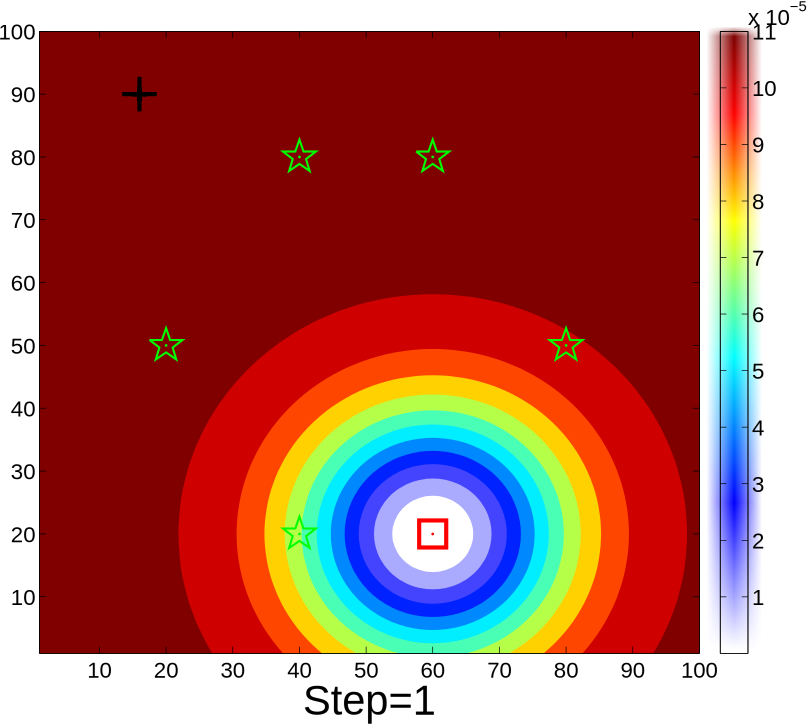
\includegraphics[width=\textwidth]{figures/sta_sen_sta_tar_top1_3_dbf_first}
%			\caption{Individual PDF}\label{fig:sta_sen_sta_tar_top1_init_dbf}
%		\end{subfigure}
%		\begin{subfigure}[b]{0.21\textwidth}
%			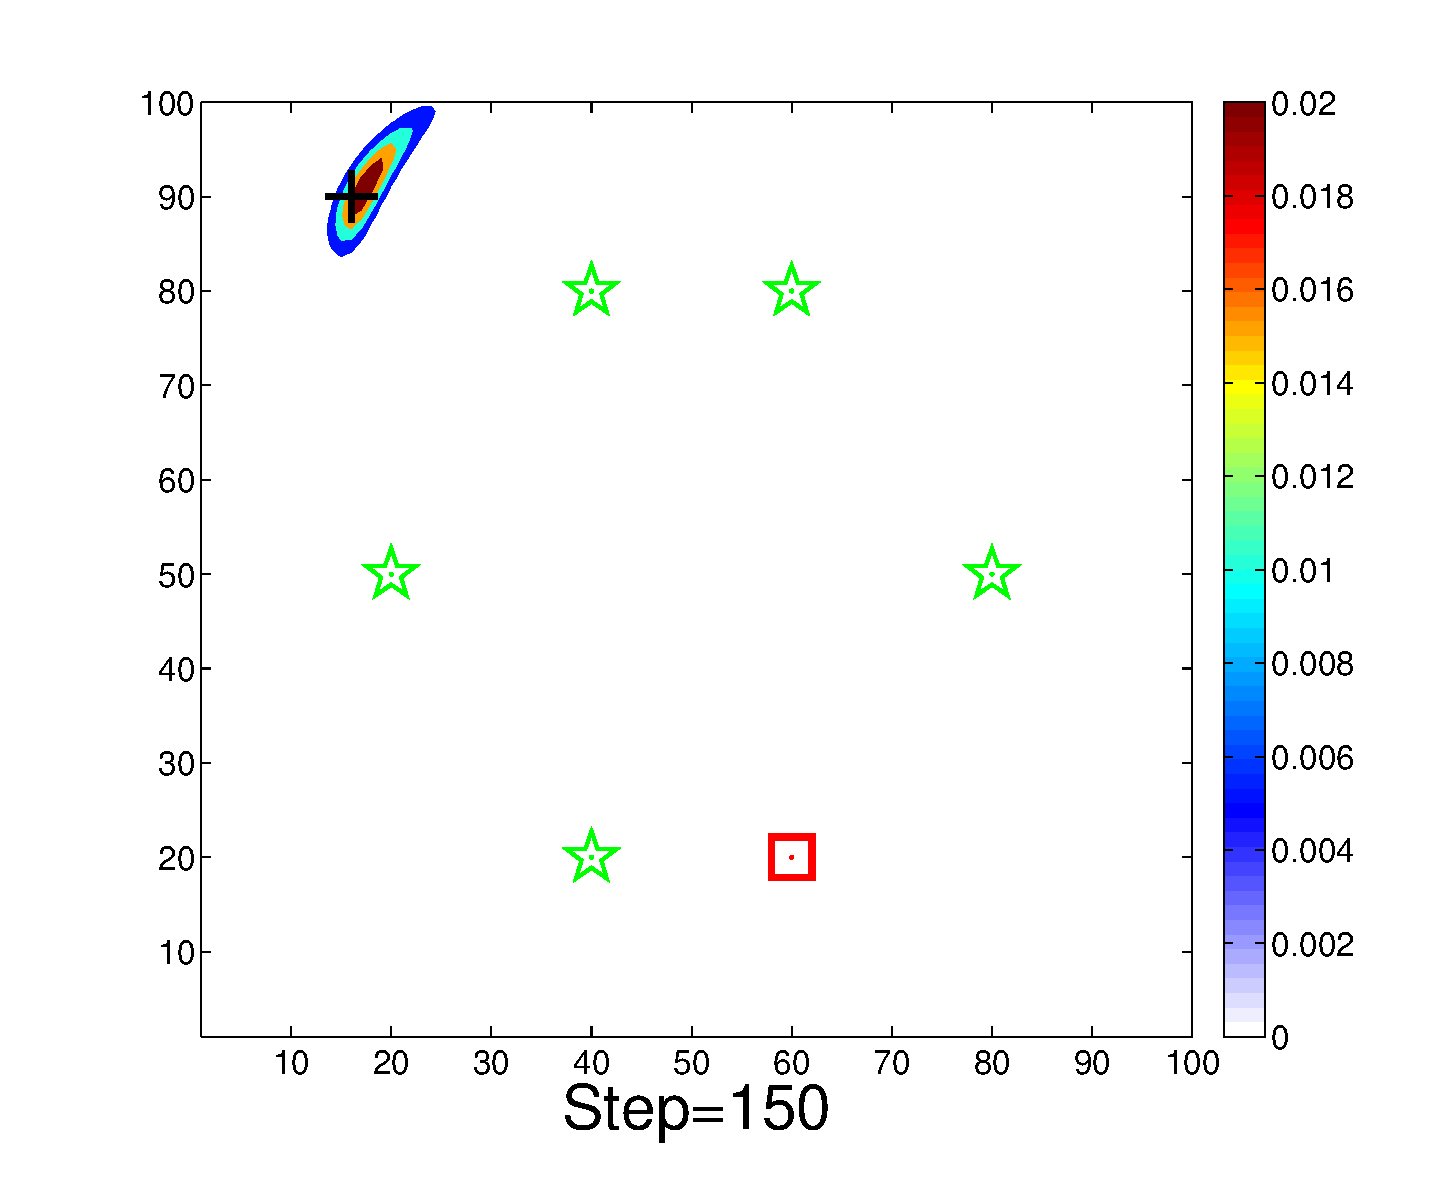
\includegraphics[width=\textwidth]{figures/sta_sen_sta_tar_top1_3_dbf_end}
%			\caption{\proto-DBF}\label{fig:sta_sen_sta_tar_top1_dbf}
%		\end{subfigure}
%		\begin{subfigure}[b]{0.21\textwidth}
%			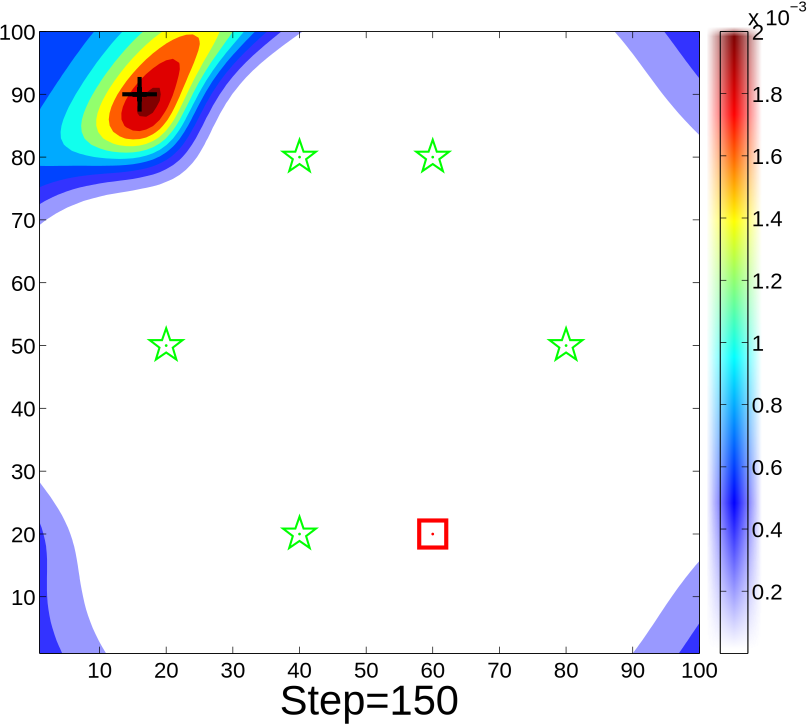
\includegraphics[width=\textwidth]{figures/sta_sen_sta_tar_top1_3_cons_end}
%			\caption{Consensus method}\label{fig:sta_sen_sta_tar_top1_cons}
%		\end{subfigure}
%		\begin{subfigure}[b]{0.21\textwidth}
%			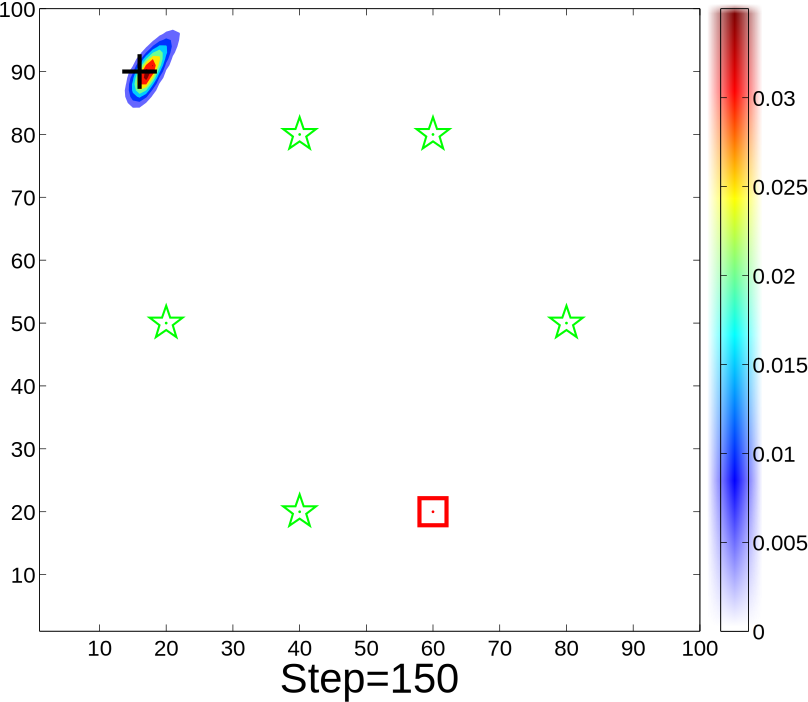
\includegraphics[width=\textwidth]{figures/sta_sen_sta_tar_top1_cent_end}
%			\caption{Centralized filter}\label{fig:sta_sen_sta_tar_top1_cent}
%		\end{subfigure}	
%		\begin{subfigure}[b]{0.23\textwidth}
%			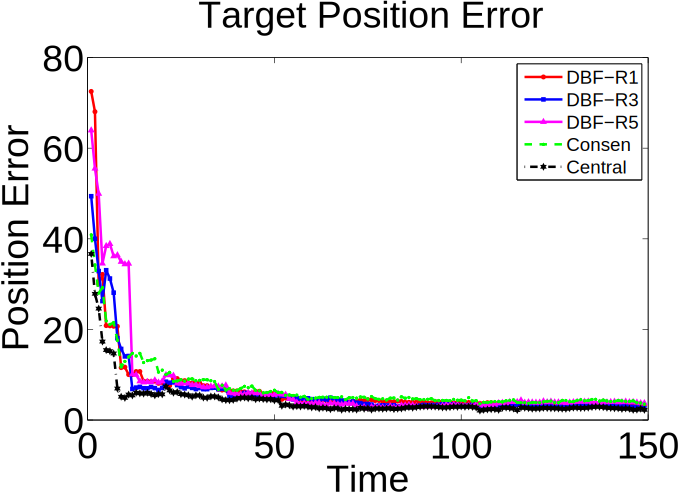
\includegraphics[width=\textwidth]{figures/sta_sen_sta_tar_top1_pos_err}
%			\caption{Position error}\label{fig:sta_sen_sta_tar_top1_pos_err}
%		\end{subfigure}	
%		\begin{subfigure}[b]{0.23\textwidth}
%			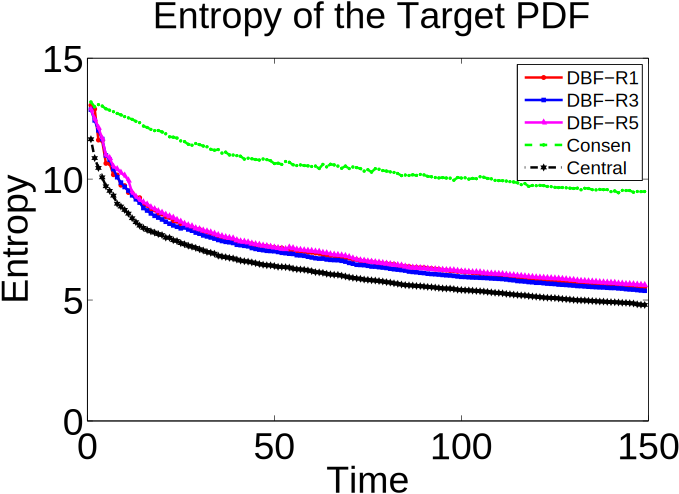
\includegraphics[width=\textwidth]{figures/sta_sen_sta_tar_top1_entropy}
%			\caption{Entropy reduction}\label{fig:sta_sen_sta_tar_top1_entropy}
%		\end{subfigure}		
%		\caption{First scenario: (a) two types of topologies; (b) individual PDF of the $3^\text{rd}$ UGV after initial observation; (c)-(e) PDFs at the end of simulation using different filters; (f) average position estimation errors; (g) average entropy of PDF. In last two figures, metrics are based on the PDFs of the $1^\text{st}$, $3^\text{rd}$ and $5\thi$ UGV using \proto-DBF, the common PDF using CbDF and using CF.}
%		\label{fig:sta_sen_sta_tar1}
%		\vspace{-1.3em}
%	\end{figure}
%	
%	In the first scenario, each UGV forms a circular individual PDF after the initial observation, centered at its own position, as shown in \cref{fig:sta_sen_sta_tar_top1_init_dbf}.
%	The circular PDF occurs because the sensor model only depends on the relative distance between a UGV and the target, not on the relative bearing.
%	As more observations are received by each UGV, the posterior individual PDF concentrates to the true location of the target (\cref{fig:sta_sen_sta_tar_top1_dbf}), which accords with the consistency of \proto-DBF.	
%	
%	Comparison of the estimation performance between \proto-DBF, CbDF and CF is presented in \cref{fig:sta_sen_sta_tar_top1_pos_err,fig:sta_sen_sta_tar_top1_entropy}.
%	Unsurprisingly, the CF achieves the best performance in terms of both small position estimation error and fast reduction of entropy. 
%	This happens because the central unit has access to the latest observations of all UGVs, thus making most use of all available information.
%	\proto-DBF and CbDF show similar performance as the CF does in position estimation error.
%	However, they significantly differ in terms of entropy reduction. 
%	In fact, \proto-DBF has similar asymptotic performance as the CF in reducing the entropy of PDF over time; this is notable since each UGV only communicates with its neighboring UGVs, which consumes less communication recourse than the CF.
%	The CbDF, on the contrary, is much slower in entropy reduction while incurring huge communication burden due to multiple rounds of consensus at each time step.
%	The difference in entropy reduction makes sense since CbDF can only ``implicitly" fuses different robots' observation via computing the average of individual PDFs while \proto-DBF and CF can directly utilize observations, thus making better use of available information.	
%	Such difference results in vastly different individual PDFs, as shown in \cref{fig:sta_sen_sta_tar_top1_dbf,fig:sta_sen_sta_tar_top1_cons,fig:sta_sen_sta_tar_top1_cent}, which show the PDF at the end of simulation.
%	Similar performance difference among \proto-DBF, CbDF and CF for the second scenario can be observed in \cref{fig:sta_sen_sta_tar2}.
%		
%	\begin{figure}%[thpb]
%		\centering
%		\begin{subfigure}[b]{0.45\textwidth}
%			\includegraphics[width=\textwidth]{figures/com_topo2}
%			\caption{Collection of changing topologies}\label{fig:com_topo2}
%		\end{subfigure}
%		~
%		\begin{subfigure}[b]{0.21\textwidth}
%			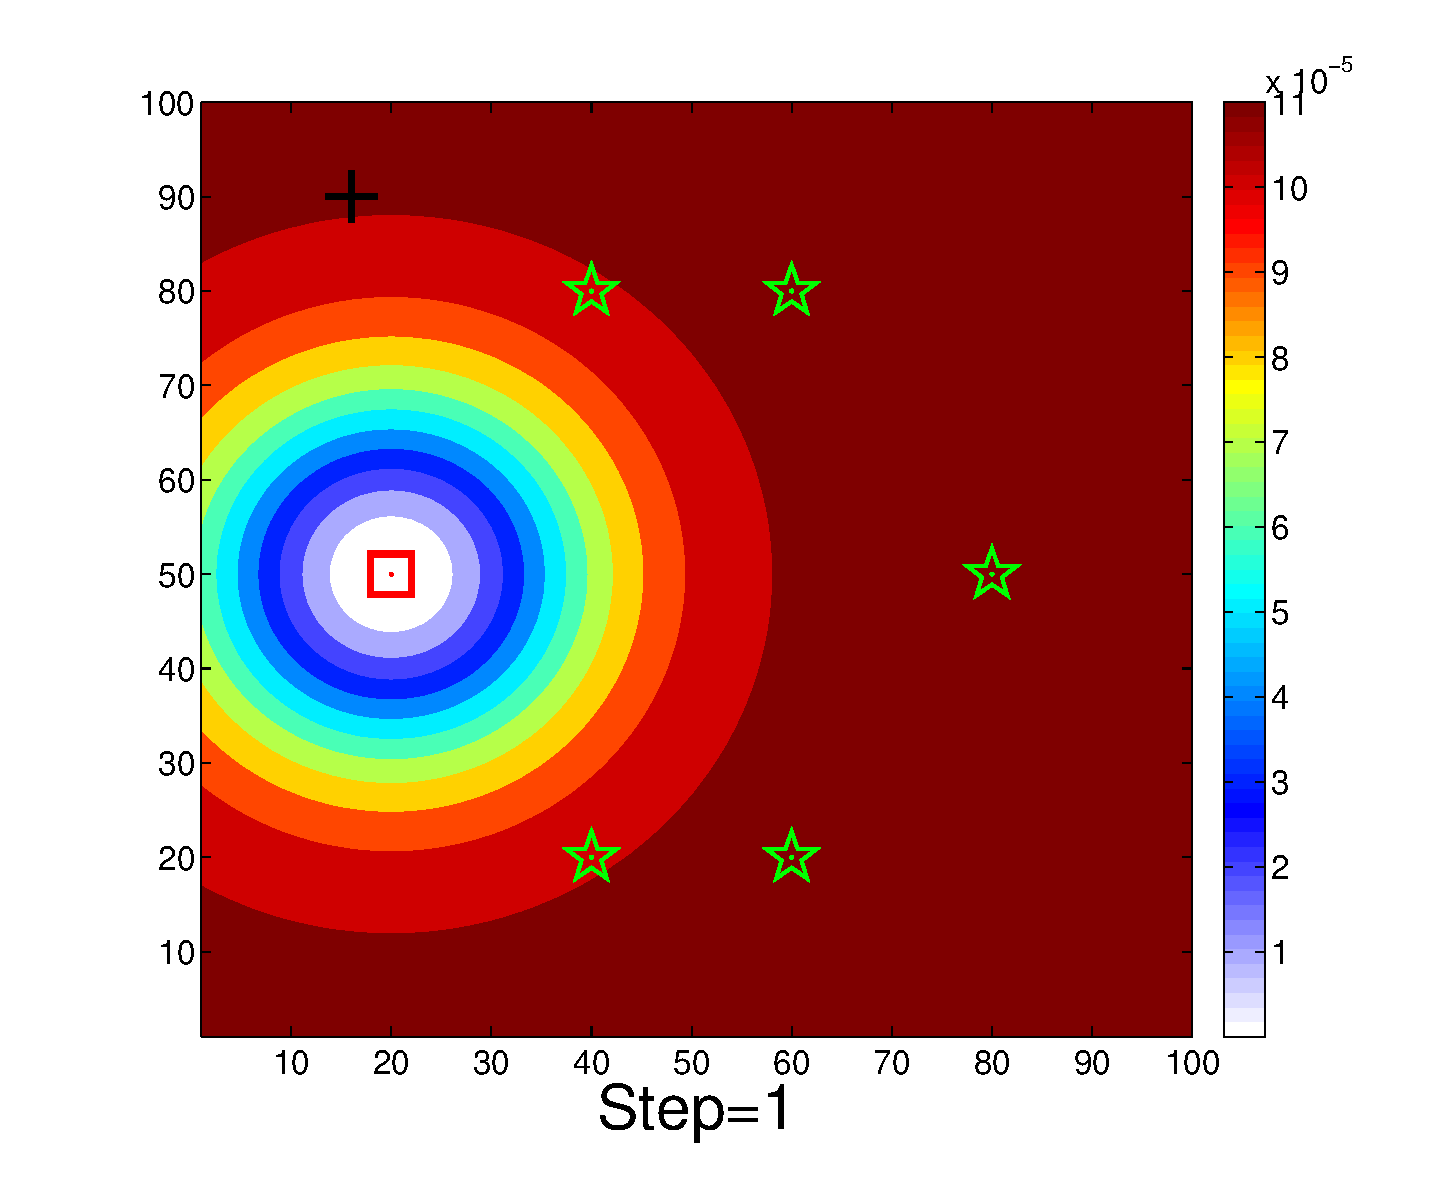
\includegraphics[width=\textwidth]{figures/sta_sen_sta_tar_top2_1_dbf_first}
%			\caption{Individual PDF}\label{fig:sta_sen_sta_tar_top2_init_dbf}
%		\end{subfigure}
%		\begin{subfigure}[b]{0.21\textwidth}
%			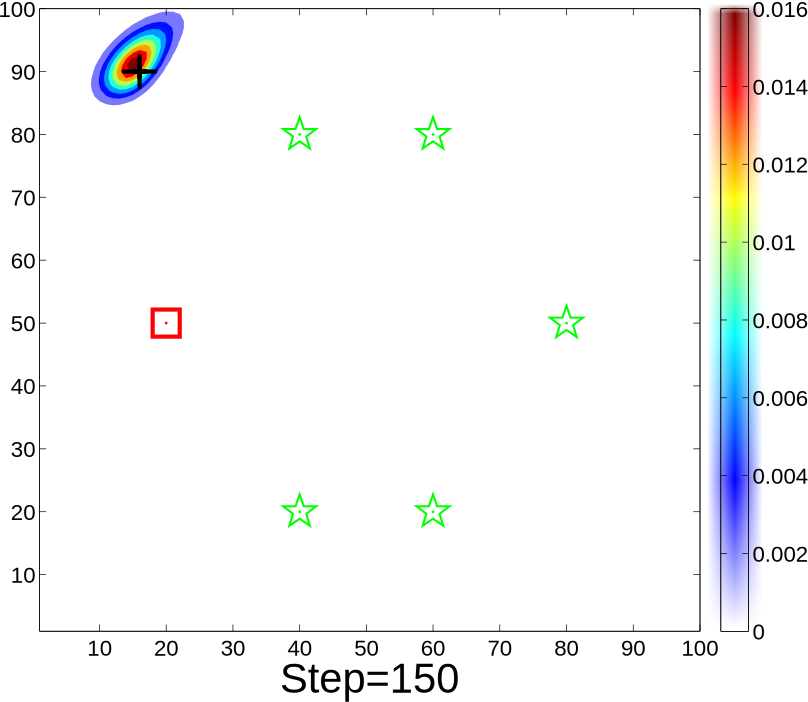
\includegraphics[width=\textwidth]{figures/sta_sen_sta_tar_top2_1_dbf_end}
%			\caption{\proto-DBF}\label{fig:sta_sen_sta_tar_top2_dbf}
%		\end{subfigure}
%		\begin{subfigure}[b]{0.21\textwidth}
%			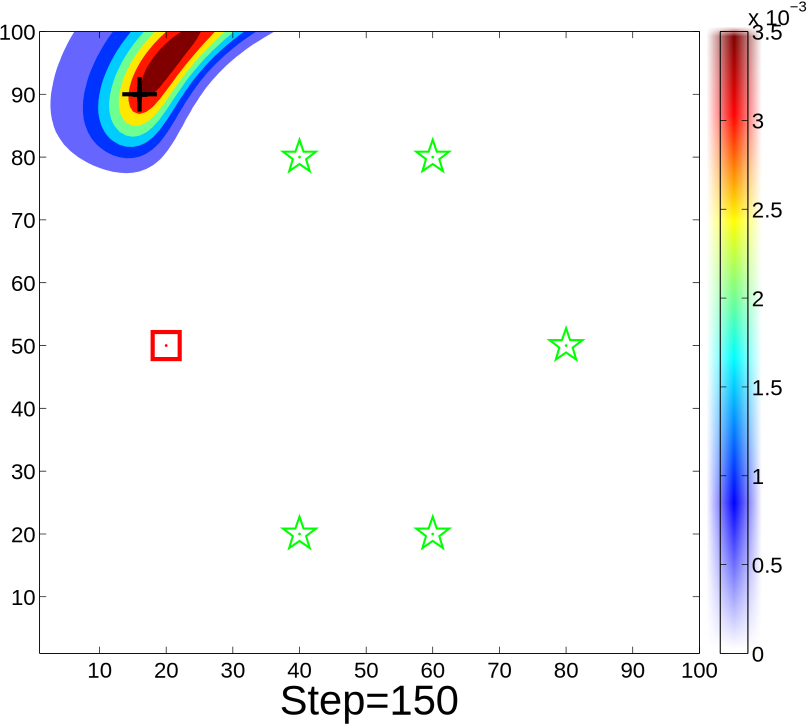
\includegraphics[width=\textwidth]{figures/sta_sen_sta_tar_top2_1_cons_end}
%			\caption{Consensus method}\label{fig:sta_sen_sta_tar_top2_cons}
%		\end{subfigure}
%		\begin{subfigure}[b]{0.21\textwidth}
%			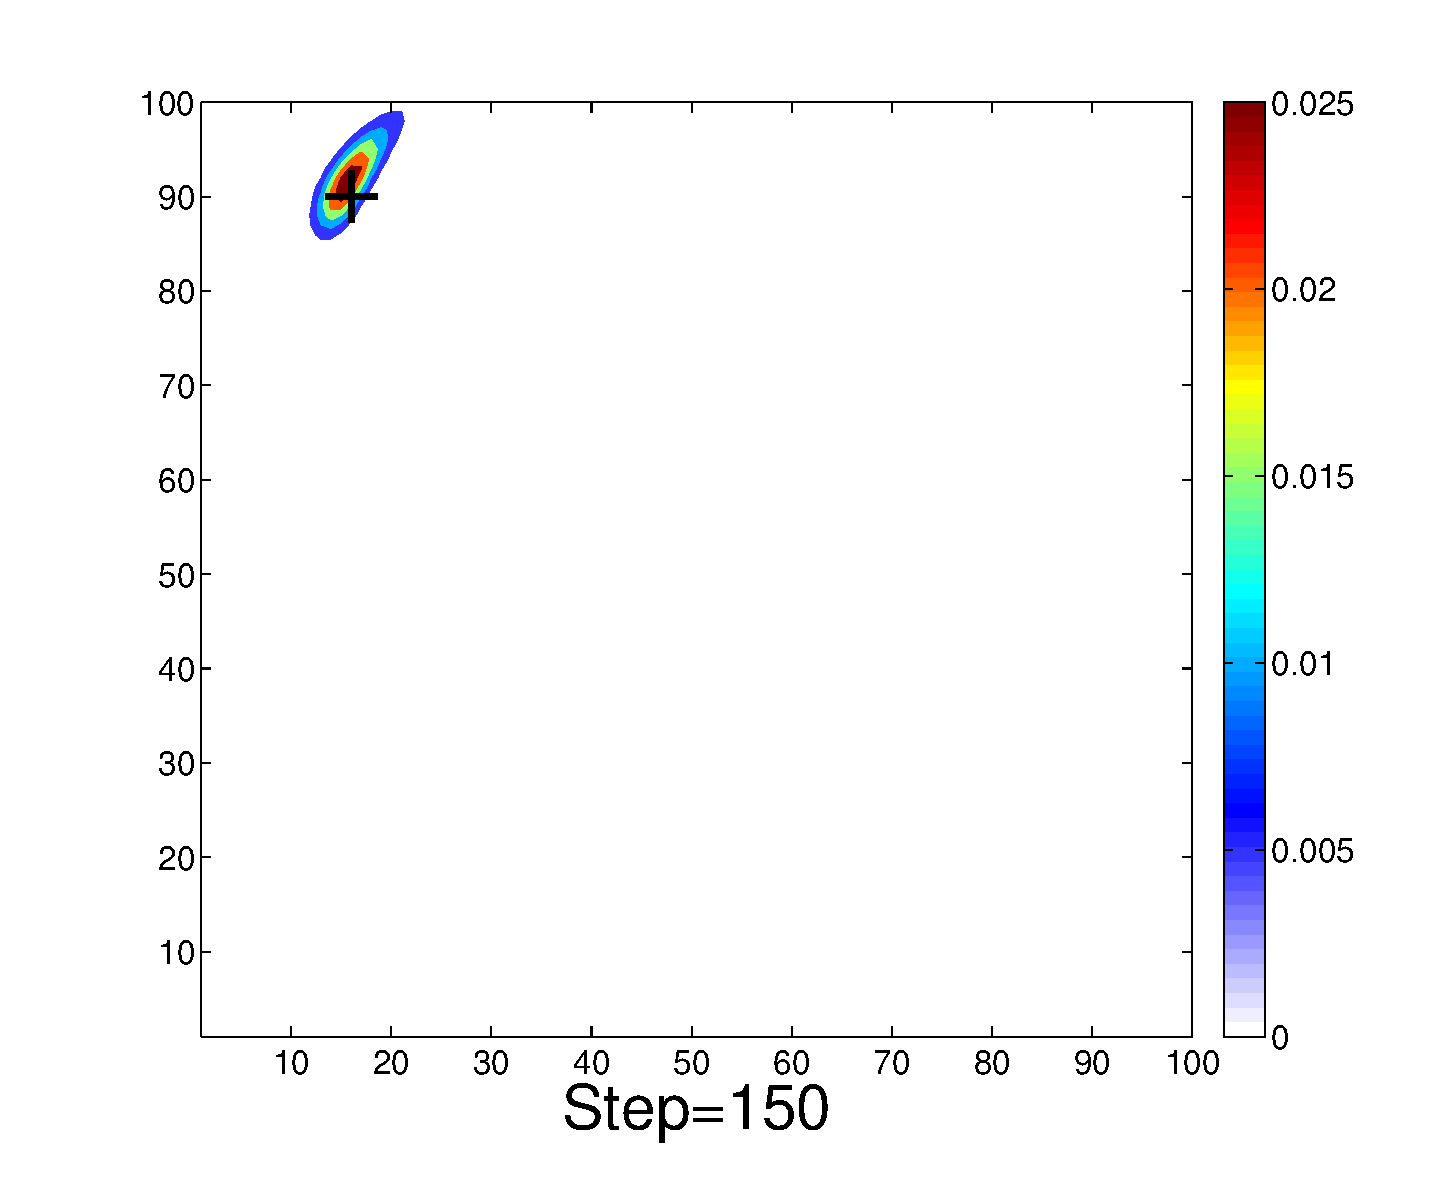
\includegraphics[width=\textwidth]{figures/sta_sen_sta_tar_top2_cent_end}
%			\caption{Centralized filter}\label{fig:sta_sen_sta_tar_top2_cent}
%		\end{subfigure}	
%		\begin{subfigure}[b]{0.23\textwidth}
%			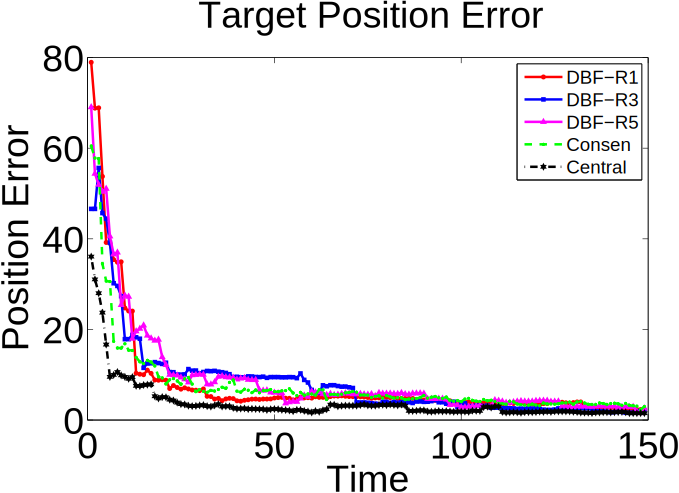
\includegraphics[width=\textwidth]{figures/sta_sen_sta_tar_top2_pos_err}
%			\caption{Position error}\label{fig:sta_sen_sta_tar_top2_pos_err}
%		\end{subfigure}	
%		\begin{subfigure}[b]{0.23\textwidth}
%			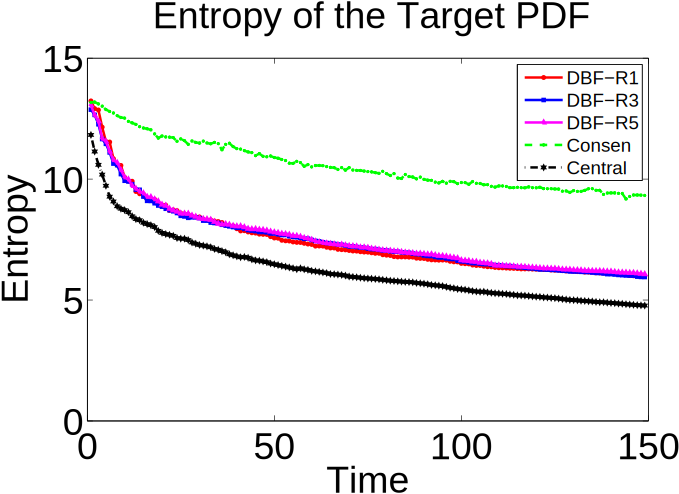
\includegraphics[width=\textwidth]{figures/sta_sen_sta_tar_top2_entropy}
%			\caption{Entropy reduction}\label{fig:sta_sen_sta_tar_top2_entropy}
%		\end{subfigure}		
%		\caption{Second scenario consists of three types of topologies. (b)-(d) show individual PDFs for $1^\text{st}$, $2^\text{nd}$ and $5\thi$ UGV, respectively.}
%		%			Individual PDFs for three switching interaction topologies: (b)-(e) The $1^\text{st}$ UGV's individual PDFs; (f)-(i) The $2^\text{nd}$ UGV's individual PDFs; (j)-(m) The $5^\text{nd}$ UGV's individual PDFs. }
%		\label{fig:sta_sen_sta_tar2}
%		\vspace{-1.3em}
%	\end{figure}
		
	\section{Conclusion}\label{sec:conclu}	
	This paper presents a general measurement dissemination-based distributed Bayesian filter (DBF) method for a network of multiple unmanned ground vehicles (UGVs) under dynamically changing interaction topologies.
	The information exchange among UGVs relies on the Full-In-and-Full-Out (\proto) protocol, under which UGVs exchange the communication buffers and track lists with neighbors.
	Under the condition that the union of the interaction topologies is \fc, {\proto} can disseminate measurements over the network within finite time. 
	By using the track list, the CBs can be trimmed without causing information loss.
	The \proto-DBF algorithm is developed to estimate individual probability density function for target localization. 	
	The \proto-DBF can significantly reduce the transmission burden between each pair of UGVs compared to the statistics dissemination methods.
	Simulations comparing \proto-DBF with consensus-based distributed filters (CbDF) and the centralized filter (CF) show that \proto-DBF achieves similar performance as the CF and superior performance over the CbDF.
	
%	In our future work, we will modify the {\proto} to handle the changing number of UGVs. 
%	We will also look into the combination of transmission of measurements and parameterized statistics to save communication cost without sacrificing estimation accuracy.
%	\begin{keywords} 
%		Multiple vehicle system, target localization, environmental sensing, distributed filtering, switching interaction topology
%	\end{keywords}
	%%%%%%%%%%%%%%%%%%%%%%%%%%%%%%%%%%%%%%%%%%%%%%%%%%%%%%%%%%%%%%%%%%%%%%%%%%%%%%%%
	
%	\balance
	
%	\addtolength{\textheight}{-12cm}   % This command serves to balance the column lengths
	% on the last page of the document manually. It shortens
	% the textheight of the last page by a suitable amount.
	% This command does not take effect until the next page
	% so it should come on the page before the last. Make
	% sure that you do not shorten the textheight too much.
	
	%%%%%%%%%%%%%%%%%%%%%%%%%%%%%%%%%%%%%%%%%%%%%%%%%%%%%%%%%%%%%%%%%%%%%%%%%%%%%%%%
	
	
	
	%%%%%%%%%%%%%%%%%%%%%%%%%%%%%%%%%%%%%%%%%%%%%%%%%%%%%%%%%%%%%%%%%%%%%%%%%%%%%%%%
	
	
	
	%%%%%%%%%%%%%%%%%%%%%%%%%%%%%%%%%%%%%%%%%%%%%%%%%%%%%%%%%%%%%%%%%%%%%%%%%%%%%%%%
	%\section*{APPENDIX}
	%
	%Appendixes should appear before the acknowledgment.
	
%	\section*{ACKNOWLEDGMENT}\part{
%	%This work is supported by the Embedded Humans: Provably Correct Decision Making for Networks of Humans and Unmanned Systems project, a MURI project funded by the Office of Naval Research.
%	The authors gratefully acknowledges the Office of Naval Research for supporting this work. 
%	They would also like to thank Yuting Wei in the Department of Statistics, UC Berkeley for he}r sincere help and fruitful discussion.
	
	%The preferred spelling of the word �acknowledgment?in America is without an �e?after the �g? Avoid the stilted expression, �One of us (R. B. G.) thanks . . .? Instead, try �R. B. G. thanks? Put sponsor acknowledgments in the unnumbered footnote on the first page.
	
	
	
	%%%%%%%%%%%%%%%%%%%%%%%%%%%%%%%%%%%%%%%%%%%%%%%%%%%%%%%%%%%%%%%%%%%%%%%%%%%%%%%%
	{\footnotesize\bibliographystyle{IEEEtran}}
	%\bibliographystyle{bibtex}
	\bibliography{references}
	
\end{document}
